%!TEX root = ../thesis.tex
%*******************************************************************************
%*********************************** First Chapter *****************************
%*******************************************************************************

\chapter{Deforestation and the role of institutions and environmental policies in the Brazilian Legal Amazon}  %Title of the First Chapter

\ifpdf
    \graphicspath{{Chapter1/Figs/}{Chapter1/}}
\else
    \graphicspath{{Chapter1/Figs/}{Chapter1/}}
\fi

\begin{abstract}
This study investigates the impact of environmental legislation and environmental institutions on deforestation in the Brazilian legal Amazon. More specifically, we construct municipality level panel data for the period 2004 to 2015.  Our estimated results show that environmental policies and the expansion of key commodity markets, when conditioned on the institutional environmental framework (IEF), can be effective in curbing deforestation. Additionally, we conduct a spatial analysis which endorses our main findings. Counter-factual simulations indicate that the current institutional environmental framework has resulted in an decrease in deforestation of around 63$\%$. \\
\textbf{Keywords}: Deforestation; Environmental Policy; Market Expansion; Institutions \\
\\
JEL classification: Q23; Q28.
\end{abstract}


%********************************** %First Section  **************************************
\section{Introduction}
\label{S:1}

Forests are integral to any global carbon management and sequestration strategy and play a major role in global climatic regulation. In the context of climate change, deforestation is recognised as the second major cause of greenhouse gas emissions. With Brazil being home to over 64 per cent of the Amazon rainforest it has faced significant deforestation for more than 5 decades it is therefore important to understand what drives deforestation and hence the effectiveness of various government policies and institutions that have been introduced in an attempt to reduce it. Historically, the main causes for deforestation in Brazil are transport infrastructure, settlement expansion, agricultural expansion, and cattle ranching (\citet{GEIST2}, \citet{PFAFF3}, \citet{NEPSTAD} and \citet{RICHARDS}). To prevent further deforestation Brazil has implemented a number of environmental legislation and regulatory institutions. The purpose of this study is to investigate to what extent this new institutional environmental framework (IEF) has been successful in curbing the loss of rainforest in Brazil by examining the determinants of Brazilian deforestation for the period 2004-2015. Our main contribution is to investigate the impact of both the expansion of the beef, soy and forest product markets and the effectiveness of Brazil's policies to protect the Legal Amazon conditional on the institutional environmental framework in place at the time.\footnote{The Legal Amazon is an area that corresponds to 59$\%$ of the Brazilian territory and encompasses all eight states (Acre, Amapá, Amazonas, Mato Grosso, Pará, Rondônia, Roraima and Tocantins) and part of the State of Maranhão (west of the meridian Of 44ºW), totalling more than 5 million km$^{2}$. The concept of Legal Amazon was established in 1953 and its territorial limits stem from the need to plan the economic development of the region and, therefore, are not limited to the ecosystem, which occupies 49$\%$ of the national territory and also extends into the territory of eight neighbouring countries \citep{IPEAwebsite}.} 

Our study is at the municipality level where we have detailed information on 562 municipalities where we are able to control for a wide range of possible determinants of deforestation. Our methodological approach is to employ a panel fixed effects regression model that takes into account environmental policies and prices, and the underlying institutional environmental framework. Following \citet{assuncao2015} a second contribution is to quantify what the level of deforestation may have looked like had Brazil not implemented its current institutional environmental framework.

The rates of deforestation in the Brazilian Amazon as well as the reasons behind them have varied considerably over time. In the late 60's there was substantial investment in transport infrastructure to increase the productivity of isolated regions \citep{BAYNARD}. In addition, the government identified land settlement as one of its priorities, benefiting both the landless poor and southern Brazilian agribusiness \citep{CALDAS,DIPROSE}. During the 1970s, Brazil's policy shifted from rapid frontier colonisation to agrarian reform schemes as a strategy to reverse the tendency of land concentration into large landholdings from the migrants coming from the south of Brazil and the internationalisation of the Amazon region.  Part of this reform process involved the creation of the Brazilian Institute of Agrarian Reform (IBRA in Portuguese) and the National Institute of Agrarian Development (INDA in Portuguese), later replaced by the Institute for Rural Settlement and Agrarian Reform (INCRA in Portuguese). The causes of deforestation changed in the 1980s and were largely driven by the need for land to satisfy the global demand for cattle and soy production \citep{CROPPER1,SOLER}.

By the end of the 20th century, the Brazilian government indirectly encouraged deforestation in the Amazon through the national land reform program introduced by the INCRA that promoted various colonisation schemes in areas close to newly built highways. During this process, for so-called agricultural pioneers, access to credit and subsidies for agriculture and pasture were increased especially along the deforestation line that ran next to major road arteries (for example, the BR 153 "Belem - Brasilia" and the BR 364 "Cuiaba - Porto Velho"). The process of deforestation was further accentuated by the construction of federal roads, mining, and hydroelectric projects. Such actions eventually came to the attention of international organisations who, in turn, exerted pressure on the Brazilian government to reduce levels of deforestation. As a result, the government introduced a series of measures to curb deforestation through combination of environmental policies reinforced by a new environmentally focussed institutions.

Hence, in the early 2000s, Brazil's National Environmental System (SISNAMA in Portuguese) changed the National Environmental Policy (Pol\'{i}tica Nacional do Meio Ambiente in Portuguese) on deforestation to a more decentralised operation with the hope that this would result in increases in both effectiveness and efficiency. To this end, the National Environmental Policy (NEP) aggregated federal, state, and local government bodies to form, what we call in this paper, Brazil's institutional environmental framework (IEF). Two of the local institutional actions were the implementation of environmental laws and establishment of environmental offices in municipality city halls.  The explicit role of these new offices was to formulate and execute policies related to the environment and to control, monitor, evaluate, and execute the management of the natural resources within a municipality in accordance with the local environmental legislation. One should note, however, that many municipalities chose not implement this action and would often designate this role to other existing offices (with different core agendas).

Although the NEP covers all of Brazil, given that much of the world's tropical forests lie within the region defined as the Legal Amazon, the focus of the policy was on this region. In accordance with the NEP, in 2004 the government created the Action Plan for the Prevention and Control of Deforestation in the Legal Amazon (PPCDAm in Portuguese). Its purpose is to plan development, control land use and ensure compliance with the environmental law and promote sustainable practices. In order to control land use and prevent further deforestation, the PPCDAm  also includes the satellite-based monitoring programme PRODES (Projeto de Estimativa do Desflorestameno da Amaz\^{o}nia in Portuguese) \citep{inpe} that attempts to record incidents of deforestation throughout the year within the policy area. All the data gathered by the action plan are used to enforce the PPPCDAm plan, which includes the issuing of fines for agents who clear or damage the forest, embargoes of areas in the process of being cleared with the confiscation of equipment, and restrictions on access to subsidised credit \citep{AUBERTIN}.\footnote{In order to control for degradation of the forest by selective logging and forest fires, the government uses the DETER program. In addition, two other systems were introduced in 2007: DEGRAD (Mapeamento da Degradaç\~{a}o Florestal na Amaz\^{o}nia Brasileira in Portuguese), for mapping forest degradation in the Legal Amazon, and DETEX (Mapeamento da Cobertura Florestal na Amaz\^{o}nia Brasileira in Portuguese), for detecting logging operations in the Legal Amazon region \citep{VALERIANO}.} As a further environmental policy to limit the expansion of cleared land the PPCDAm also established a series of Protected Areas (PA) which are defined as areas that represent ecological mosaics and corridors, considered essential for conserving biodiversity and traditional communities, as well as being providers of environmental services for the generation of business opportunities.\footnote{The Law on the National Register of Conservation Units (Sistema Nacional de Unidades de Conservacao (SNUC)) dates from 2000. It defines 12 different types of unit. In general, conservation units are territorial spaces, including their environmental resources, with relevant natural characteristics, which have the function of ensuring the preservation of the biological patrimony. There are 334 conservation units operating in the Legal Amazon in 2017, of which more than two thirds are classified as conservational sustainable use units which differ from standard conservation units due to the existence of traditional populations that contribute to the development of sustainable economic activities, if we add the indigenous lands, nearly 50\% of Amazonian land area is protected \citep{AUBERTIN,MMA,MMA2017}. In this paper we classify indigenous land and conservational units as protected areas.}

Despite the formation of both institutions and policies to deal with deforestation in Brazil, much of the literature that analyses the determinants of deforestation and the effectiveness of environmental policy only considers the role of institutions in terms of action plans at an aggregate level and land tenure insecurity and property rights at the more disaggregated level \citep{ARAUJO, OLIVEIRA2}. \citet{BORGES} examine the problem of deforestation in the Amazonian region and the role of the Brazilian government regarding local environmental governance and public policies. The study identified some participatory-based, decentralized models of forest management and existing forest regulatory frameworks which showed how local environmental governance can become operative and serviceable for a sustainable balance between the use of natural resources, conservation and regional planning. \citet{NEPSTAD} highlighted the impact of institutional factors, such as enforcement of laws, intervention in the soy and beef supply chains, restrictions on access to credit, and expansion of protected areas, all of which are found to have contributed to a decline in the demand for new deforestation in the Brazilian Amazon \citep{NEPSTAD}. In addition, \citet{VALENTIM2} found that the deforestation was not significantly related to environmental governance which included many different governance dimensions and didn't control for environmental policies and market prices. More recently, \citet{pailler_2018} investigated how local political processes create incentives to manipulate forest resources and shows that local electoral processes lead to increased deforestation in the Brazilian Amazon. The author pointed out that electoral deforestation cycles do not appear to be driven by changes in agricultural policy implementation and activity, but are linked to corruption and campaign finance, suggesting that weak institutional constraints facilitate electoral manipulation of forest resources.

Although these previous studies emphasize the role of institutions in different levels and policy intervention, little has been done concerning the impact of the policy expansion on reducing deforestation and how their effectiveness may be affected by the presence of municipality level institutions for managing environmental policy while controlling for market expansion which is the main driver of deforestation at the present. It is, thus, imperative to study the institutional framework undertaken at the minimum level taking into account the different causes for the process of deforestation in Brazilian Amazon. Our study contributes to the existing literature by analysing the role played by Brazil's IEF. In addition, we take one step further in analysing the spatial context of the IEF in the Legal Amazon over the studied period.

To briefly summarise our results, we find that the creation an institutional environmental framework (IEF) whilst a positive step, was undermined by weak enforcement such that the introduction of environmental laws as an instrument of the NEP had little impact on deforestation. However, municipalities who created an environmental office did experience a reduction in the deforestation rate when combined with environmental policies and taking into account an expansion of the market for key commodities. We conduct a spatial analysis taking into consideration the spatial dependence assumption for deforestation process \citep{hargrave_kis-katos_2012} and, in our results, we find that the existence of an IEF within municipality has a negative spillover effect on neighbouring municipalities. On counter-factual simulations to quantify the amount of forest that would have been cleared, had there been no institutional environmental framework show that deforestation would have been approximately 63$\%$ more than it was if there had been no institutional environmental framwork. Following \citet{assuncao2015}, the monetary benefits of avoiding deforestation and protecting the forest show that the preserved forest area is worth the equivalent to 12 billion tonnes of stored $CO_{2}$ with an estimated value of US\$\ 62b.

The reminder of the paper is organized as follows.  Section 2 describes the conceptual framework and outlines the main testable hypotheses.  Section 3 describes the data and our empirical approach.  Section 4 presents the results of our main regressions while Section 5 provides a series of counter-factual simulations.  Section 6 concludes.


%********************************** %Second Section  *************************************
\section{Conceptual Framework}
\label{S:2}

\subsection{Main Hypothesis}
\label{SS:2}

Our analytical approach is to include Brazil's institutional structure within the framework suggested by \citet{ANGELSEN4} and \citet{hargrave_kis-katos_2012}. As the Legal Amazon is often thought of as a frontier region it is often considered open access land in which deforestation depends positively on the expected profits from using the land for unsustainable activities, such as logging, cattle ranching or farming.\footnote{According to Brazilian Forest Service data, by December 2015 there were 68.8 million hectares of forests awaiting allocation for the recognition of indigenous lands and traditional communities, as well as conservation units \citep{SFB,Imazon2017}.} Moreover, in the Legal Amazon region land use decisions are made taking into account the expected profit differential between sustainable (such as protected areas (PAs)) and unsustainable land use \citep{hargrave_kis-katos_2012}. We assume that the services from sustainable land use are public goods and thus are ignored by the agents when deciding what land to clear \citep{ANGELSEN4}. In this sense, agents maximise expected profits by choosing the amount to clear under certain constraints.

Hence, the expected profits of land use are determined by the prices of agricultural and forestry goods, access to markets, and other municipality specific conditions. Deforestation costs are given by the costs of clearing the land, agricultural and cattle ranching costs, the opportunity to obtain credit and the risk of being fined for illegal forest clearing \citep{hargrave_kis-katos_2012}. In addition, it is believed that agents who are aware of satellite monitoring choose cloudy days to clear the unsustainable land, suggesting a positive correlation between deforestation and cloud cover \citep{CALIXTO}.

We conjecture that the existence of an institutional framework affects agents' forest clearing decision. The term institutional is defined as a code of practice, behaviour, or relationship that has significant tangible or intangible social outcome, such as socioeconomic and environmental sustainability \citep{NORTH}. Often such relationships, behaviours, or practices are facilitated by physical organisations and/or actors, sanctions or rewards. In this sense, the concept of an institution incorporates policies and legislation. Strong institutions have the potential to decelerate the clearing process through the enforcement of environmental laws and through the management of environmental policies. For example, the risk of being penalised for clearing a forest becomes higher when there is institutional compliance within a local area. However, the strength of any institution depends in part on political structures of a municipality, such as the political party, education of the mayor, the level of existing corruption, or the election process.\footnote{When dealing with developing countries it is important to account for the fact that more regulation may provide government officials with more levers for extracting rents. Hence, it is necessary to include controls for government efficiency. One approach is to capture the possibility of corruption occurring in a system. \citet{BROLLO_2013} identified that larger federal transfers from the FPM (Fundo de Participacao Municipal in Portuguese) increased observed corruption. \citet{BUGARIN} found that the existence of commissioned workers in the Brazilian government leaded to corruption in the Executive body. Corruption in this work is considered a behaviour associated with a particular motivation, which is to obtain a private gain at the public expense. In this sense, corruption arises whenever an agent, who is responsible for certain public responsibilities, and is influenced by the prospect of some reward, performs actions in favour of those who provide such reward, and therefore harms the public to whom such an individual should respond \citep{CARL2002}. The existence of corruption within the municipality governmental infrastructure is related to the benefits and costs of an unlawful act since each agent intends to maximise its utility. The costs are determined by the probability of detection of the action and by the severity of the punishment, which may be either loss of popularity for politicians, wages, employment, and also the possibility of being prosecuted and imprisoned. The benefits are related to the financial gain \citep{GARCIA, ALBUQUERQUE, BUGARIN} or the possibility of being reelected \citep{BROLLO_2013}.} 

If institutions are fragile, the agents have more incentives to misappropriate revenues \citep{GARCIA, ALBUQUERQUE, BROLLO_2013, BUGARIN}. In addition, how well the institutional apparatus works in a municipality is also likely to determine the preservation and maintenance of sustainable lands \citep{ROCHEDO2018}. Our framework, then, assumes that the determinants of the expected profits are divided into market conditions, policy pressure, predetermined conditions, and institutional factors.

%We consider market conditions by capturing commodity prices (meat and soy). If these prices increase, there should be an increase in deforestation. For forestry products price, intuitively it may lead to an increase in deforestation due to high prices but it might incentivise investments in forestry products, thus contributing to the conservation of forestry to posterior clearing and then decrease deforestation.

%Policies in general can affect the expected profits from deforestation. Environmental policies constitute a risk factor for clearing, whereby transgressing an environmental policy has a negative effect on the expected profitability of clearing and thus a decreasing effect on deforestation. Additionally, some environmental policies, as for example in protected areas, serve as barrier to deforestation but could also be ineffective if they are located in areas where the deforestation pressure is low and, at the same time, it could respond positively if new protected areas are placed to curb deforestation in areas with high levels of deforestation as well \citep{hargrave_kis-katos_2012}.

%Economic policies such as subsidised credits can fuel deforestation by making clearing plans that result from a rise in expected profits. Settlements projects could also lead to deforestation since the colonists clear land in order to establish their ownership and also because their livelihood depends on agriculture and pasture activities. In contrast, housing projects within municipality prevent agents from clearing forest land in frontier areas.

%Strong institutional factors also have the potential to decelerate the clearing process through the enforcement of environmental laws and through the management of environmental policies such as environmental offices within a municipality under a certain political structure and the compliance of environmental laws. The impact of these institutional mechanisms depends on the level of involvement of the institutions \citep{NORTH}. Dealing with frontier regions, however, it must consider that the institutional framework might fail to ensure the compliance with the law since frontier deals with several structural problems as land tenure insecurity, for example.

%As for predetermined conditions,

\subsection{Institutional Environmental Framework}

%Decree nº 73.030/73
The development of the Brazilian IEF began during the 1970s as a response to pressure from a number of international organisations. As a result Brazil created the Special Secretariat for the Environment (Secretaria Especial de Meio Ambiente in Portuguese) with the remit to protect the environment and to regulate the rational use of the natural resources within territory under the supervision of the Interior Ministry. After a decade, it was implemented the Brazil's National Environmental System (SISNAMA in Portuguese) which represents the adopted structure of the national environmental management along with the introduction of the National Environmental Policy (NEP). At that time, municipalities did not have political and administrative autonomy and the introduction of a decentralised policy was considered to be an innovative initiative. \footnote{\citet{pailler_2018} considers the National Environmental System as a centralised central agency which differs from the assumption we make in this section. For more explanation on the Brazilian decentralised environmental system see \citet{SCARDUA2003} and \citet{SANCHES2017}.}

The National Environmental System consists of six distinctive bodies and environmental institutions each with a specific role. At the highest level, the government council consists of all ministers and the Union's legal advisers who suggest to the chief in command on environmental subjects which enables the president to formulate national policy and set the rules for the correct use of the environment and its resources.

The next level down is the environmental council that proposes governmental policy on the environment and natural resources to the governing council, and deliberates on norms and standards compatible with an ecologically balanced environment. The environmental council is a representative body which consists of five sectors, namely: federal, state and municipal bodies, the business sector and society. In this way, it is incumbent upon the environmental council to establish the federal standards and norms that must be observed by the states and municipalities. However, states and municipalities also have the authority to introduce other standards, as long as they do not violate the standards established by the environmental council. As a central body, the Ministry of Environment has to plan, coordinate, supervise, and control the national environmental policy and the governmental directives set for the environment as federal level body \citep{MENDESJUSBRASIL}. The framework is shown in Figure 1.



\begin{figure}[!h]
\tikzstyle{block} = [draw, rectangle, rounded corners, fill=lightgray!50, text width=6em, text centered, minimum height=12mm, minimum width=11mm, node distance=9em]
\tikzstyle{block2} = [draw, rectangle, fill=white, text width=6em, text centered, minimum width=5mm, minimum height=12mm, node distance=5em]
\tikzstyle{line} = [draw,-latex', thick]
\tikzstyle{block3}=[draw, rectangle, rounded corners, align=center, fill=lightgray,minimum height=15mm, minimum width=\textwidth, text width=20em, text centered]

\resizebox{1\linewidth}{!}{%
\begin{center}
\begin{tikzpicture}

\node [block3] (SISNAMA) {Brazilian Environmental System};
\node [block, below of=SISNAMA, yshift=4em, xshift=-18em] (organsuperior) {Superior \\ Body};
\node [block2, below of=organsuperior,] (government) {Government \\ Council};
\node [block, below of=SISNAMA, yshift=4em, xshift=-11em ] (organdelib) {Consultative \\ Body};
\node [block2, below of=organdelib, ] (conama) {Environment \\ Council};
\node [block, right of=SISNAMA, yshift=-5em, xshift=-13em] (organcentral) {Central \\ Body};
\node [block2, below of=organcentral,] (mma) {Ministry of Environment};
\node [block, right of=SISNAMA, yshift=-5em, xshift=-6em] (organexecutor) {Executive \\ Body};
\node [block2, below of=organexecutor] (IBAMA) {IBAMA};
\node [block, right of=SISNAMA, yshift=-5em, xshift=1em] (organdesecc) {Sectional \\ Body};
\node [block2, below of=organdesecc] (states) {States};
\node [block, right of=SISNAMA, yshift=-5em, xshift=8em] (organlocal) {Local \\ Body};
\node [block2, below of=organlocal] (munic) {Municipalities};

%arrows2

\path [line,dashed] (organsuperior) -- (government);
\path [line,dashed] (organdelib) -- (conama);
\path [line,dashed] (organcentral) -- (mma);
\path [line,dashed] (organexecutor) -- (IBAMA);
\path [line,dashed] (organdesecc) -- (states);
\path [line,dashed] (organlocal) -- (munic);

%arrows1

%\path [line] (SISNAMA) -- (organsuperior);
%\path [line] (SISNAMA) -- (organdelib);
%\path [line] (SISNAMA) -- (organcentral);
%\path [line] (SISNAMA) -- (organexecutor);
%\path [line] (SISNAMA) -- (organdesecc);
%\path [line] (SISNAMA) -- (organlocal);

\end{tikzpicture}
\end{center}
}
\caption{Organisational structure of the Brazilian Environmental System. Source: \citep{MMMAwebsite}}
\label{fig:4}
\end{figure}




At the executive level, the Brazilian Institute of Environment and Renewable Natural Resources (IBAMA in Portuguese) also known as the environmental police \citep{hargrave_kis-katos_2012} is responsible for carrying out actions of coordination, control, supervision, monitoring, and orientation to ensure the execution of actions related to environmental emergencies using instruments such as fines and embargoes. Even though the duty to act in cases of environmental emergencies encompasses all of the entities of the federation (union, states and municipalities), given the common competence established in the Federal Constitution of 1988, many municipalities and states are not equipped with the technical capabilities and police force are often unable to attend environmental incidents within their jurisdiction. In such a case, the environmental police assist these bodies at the local level to prevent deforestation \citep{SISNAMA, MENDESJUSBRASIL}.\footnote{The Federal Constitution from 1988 establishes that the environment is a fundamental right and it is classified as a public good. Therefore, the environment does not belong exclusively to a person or group, nor is it attributed to anyone who owns it.}

In terms of enforcement more generally, of the entities within the federation, states and municipalities are the sectional body and local body, respectively, and are responsible for most of the environmental control activity. Therefore, each state and municipality is required to organise its environmental control agency and environmental laws according to its needs. Finally, municipalities are legally able to exercise environmental management within their territorial limits by creating specific environmental offices and laws. In addition, municipalities have environmental police power, which legitimises them, to apply appropriate sanctions and forbid or close establishments that do not comply with the legal determinations \citep{MENDESJUSBRASIL}.

This institutional framework underpins the NEP. The purpose of the NEP is to regulate the various activities that involve the environment, which includes preservation, improvement, and recovery of environmental quality, assuring the society ways to promote the conducive sustainable development. The NEP provides policies specific to different regions of Brazil creating programs and action plans. As previously discussed, one of the most important tropical forest preservation plans was the implementation of the PPCDAm which is divided in three strategic phases.\footnote{During 2016, the Executive Board reviewed the 13 strategic objectives of Phase 3 (2012-2015) with the objective to listing strategic actions for the period 2016-2020 \citep{PPCDAM_2016}.}  In the first phase (2004-2008), the main objectives were to combat deforestation using satellite monitoring and to create a series of protected areas. Satellite monitoring meant that it was possible to notify the Brazilian environmental police (IBAMA) of environmental emergencies related to forest clearing thus enabling the police to penalise the offenders and prevent further deforestation. The action plan also allowed for the creation of conservation units and the ratification of indigenous lands as instruments of policy conservation. During the first phase, the plan also advised on territorial planning and prioritising the fight against the illegal takeover of public lands \citep{ARTAXO}.

The second phase of the PPCDAm (2008-2011) included plans to value the forest in terms of biodiversity conservation, and the forest management of timber and non-timber products. In this phase incentives were included for the monitoring of agricultural practices in deforested areas, including technological innovation and sustainable production systems. According to \citet{ARTAXO}, the second phase encouraged the implementation of the Rural Environmental Registry (Cadastro Ambiental Rural in Portuguese), an instrument through which environmental agencies geo-reference rural properties in order to qualify the remote monitoring and effectiveness of field inspection operations, as well as to guide the regularisation process for rural properties.\footnote{Many properties in the Legal Amazon did not complete the Rural Environmental Registry during the second phase of the PPCDAm delaying the process.  It was eventually concluded at the end of 2015 during the third phase of the action plan.} 

Complementing the previous phases, the third phase of the PPCDAm (2012-2015) included rules to strengthen the decentralisation of the action plan for states and municipalities through partnerships between the Union, states and municipalities, to deepen integration to further improve the prevention of environmental damage and the promotion of sustainable production systems. During the three phases, the PPCDAm plan analysed changes in municipality level deforestation with the aim of highlighting possible improvements at the local level to curb deforestation \citep{SISNAMA}.


%Currently, the states and municipalities are responsible for approximately 85$\%$ of the deforestation that occurs in the Legal Amazon. The federal level is responsible for 15$\%$ including deforestation occurring in conservational units and indigenous land \citep{SCARDUA}.


%********************************** % Third Section  *************************************
\section{Data and empirical approach}
\label{S:3}

%\subsection{Study Area}

%This study explores the municipalities included in the Legal Amazon region in Brazil. The area corresponds to approximately 5 million square kilometers across 9 states.

%Figure \ref{fig:4} illustrates the Legal Amazon pointing the pattern of deforestation according to changes in the environmental institutional regulation. It is possible to detect the changes in deforestation pattern according to changes in the environmental institutional regulation which includes environmental law and environmental office. Figure \ref{fig:4} (a) present the lack of this regulation the within the Legal Amazon and the level of deforestation in 2004. Figure \ref{fig:4} (b) shows the changes in the environmental institutional framework with the accumulative level of deforestation from 2004-2010. At Figure \ref{fig:4} (c) we can see the consolidation of the environmental institutional regulation and the path of deforestation from 2004-2015. Ultimately, the Figure \ref{fig:4} shows the magnitude of the arc of deforestation which comprises eastern, southern and southwestern area of the Legal Amazon.

%[Figure A.4]

\subsection{Data and controls}

%deforestation

%cloud and forest

This study investigates the determinants of deforestation in Brazil at the municipality level within the Legal Amazon. Figure 2 shows the Legal Amazon area that corresponds to more than 5 million square kilometers across 9 states. Our data consists of yearly observations for 562 municipalities in the Brazilian Legal Amazon delimitation from 2004 to 2015.\footnote{The Legal Amazon delimitation refers to 771 municipalities. However, in order to avoid bias introduced by municipalities with ecotone forest, we follow \citet{hargrave_kis-katos_2012} and exclude those with less than 5$\%$ of rainforest cover.  In robustness checks with also re-estimate our results using data for 10 and 15\%.}

\begin{figure}[H]
\centering
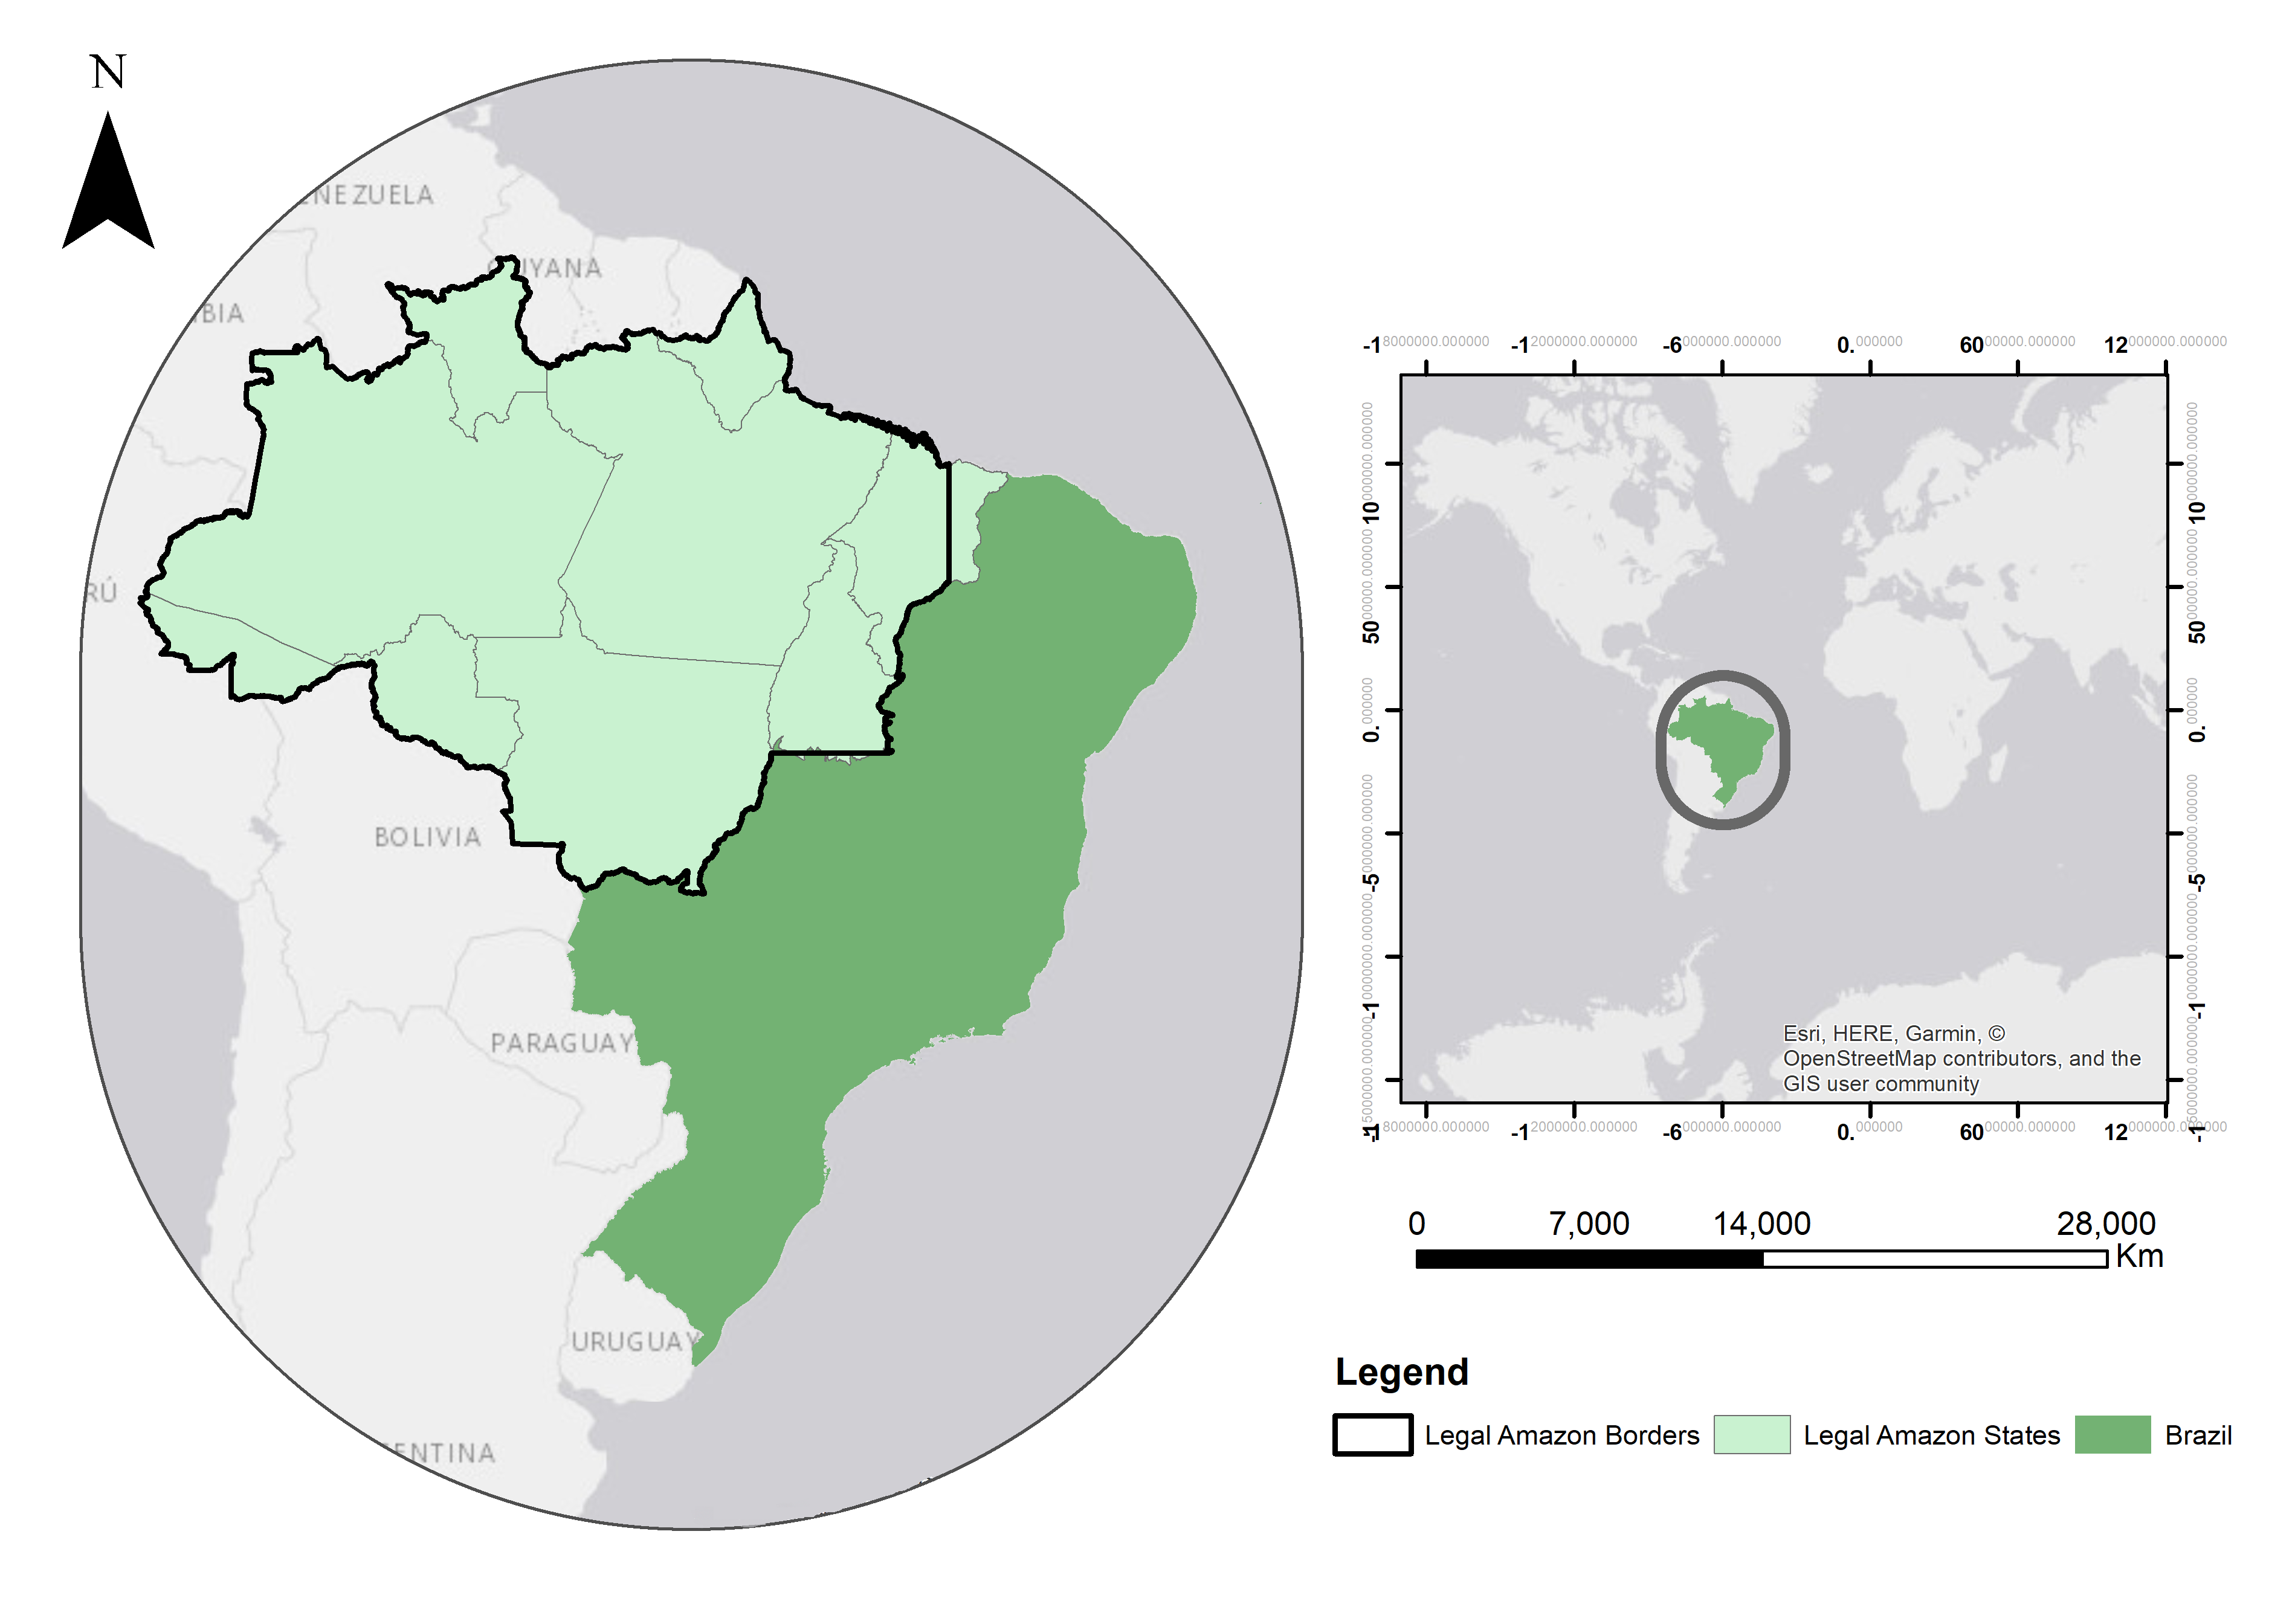
\includegraphics[width=1\textwidth, inner]{Chapter1/Chapter1_map_brazil_insect.png}
\caption[The Legal Amazon and Municipalities in the 9 states of Brazil]{The Legal Amazon and Municipalities in the 9 states of Brazil: Rond\^{o}nia, Acre, Amazonas, Roraima, Par\'{a}, Amap\'{a}, Tocantins, Maranh\~{a}o e Mato Grosso. Sources: Own construction based on data from \citet{inpe, IBGE1}}.
\label{fig:1}
\end{figure}

The data on deforestation at the municipality level comes from satellite based information from the Brazilian Institute for Space Research \citep{inpe} under the project PRODES and measures yearly deforestation in square kilometers.  The same data also gives us cloud and unobserved areas which represent the area that the satellite could not capture during a certain period. Variables for cloud and no observed areas are used in all regressions to control for measurement error related to the ability of the satellites to detect changes in the land cover across all municipalities. \footnote{According to \citet{kintisch_2007} and \citet{achard_stibig_eva_lindquist_bouvet_arino_mayaux_2010}, the PRODES estimates are considered reliable by the national and international academic science.}

Our dependent variable is the natural log of yearly deforestation within a municipality measured between July and August of any given year. We adjust all numerical variables to match the July-August year.

%beefpricecp
%soypricepp
%woodpricepp
%real gdp

To control for the expansion of commodity markets, we collect soy and wood prices at the municipality level from the Brazilian Statistical Office \citep{IBGE1}.\footnote{Wood prices come from the production of wood defined as firewood and logs of wood in cubic meters.} The beef price is reported at the state level by the Centre for Advanced Studies on Applied Economics \citep{CEPEA}. For municipalities with no data on the commodity markets, we include averaged local prices from neighbouring municipalities weighted by GDP at the municipality level, which differs from previous studies that impute zero prices for all municipalities without production of commodities in order to get the direct effect of commodity price on deforestation of commodities producing regions only \citep{hargrave_kis-katos_2012, LAKES}. We argue this approach by taking into consideration the fact that prices reflect the transport costs from each municipality to neighbouring municipalities and thus not considering averaged neighbouring municipalities price bias downward the results.
%The same procedure is applied to wood price and beef price data. We take this approach because we believe that municipalities with no commodity production still have an implicit price of commodities but this price is not higher enough to incentivise the producers.
All prices are deflated by IPCA which is the official Brazilian consumer price index. GDP is included at the municipality level to control for changes in overall economic activity \citep{IBGE1}. We gather data on federal paved roads since assist commodity activity, and there is an association between road investments and deforestation \citep{PFAFF3, CROPPER1, BAYNARD, pailler_2018}.

%mayor party
%mayor gender
%mayor educ
%mayor age
%env agency
%env law

Data on the institutional environmental framework come from the Survey of Basic Municipal Information \citep{IBGE1}. The data take the form of dummy variables that indicate whether a municipality has an environmental office and has introduced an environmental law. One important aspect that may influence whether a municipality has a well functioning environmental framework is the attitude and character of the local mayor.  Hence, we also collect data from the Survey of Basic Municipal Information on whether the political party of the mayor is pro-farmer in which may be expected to lead to greater deforestation, their education level, gender, age, and  the number of commissioned workers as a proxy for corruption since it is expected that the greater the amount of commissioned workers the higher the rate of deforestation. We also gather data from \citet{TSE} to detect mayor's re-election process. \footnote{More than 20 parties advocate the pro-farmer agenda specially in the Legal Amazon. PMDB (Partido do Movimento Democrático Brasileiro), PP (Partido Progressista), PSDB (Partido da Social Democracia Brasileira) parties respond to almost 44\% of the pro-farmer seats - bancada ruralista in Portuguese - in the deputy chambers. These political parties represent the center-right political spectrum in Brazil with the largest number of affiliates \citep{FPA}.} \footnote{According to the Survey of Basic Municipal Information commissioners workers are employees, who are not effective in the City Hall, and whose only job is the commissioned position they carry out. Usually the position is given by the mayor or city councils in exchange for political favours and benefits which proved to lead to corrupting acts \citep{BUGARIN}.} \footnote{Recently, \citet{pailler_2018} found that deforestation  rates  increased  8–10\%  in  election  years  when  an  incumbent  mayor  ran  for  re-election.}

%PSD (Partido Social Democrático), PR (Partido da Republica), PSB (Partido Socialista Brasileiro), SD (Solidariedade), DEM (Democratas), PTB (Partido Trabalhista Brasileiro), PMB (Partido da Mulher Brasileira), PDT (Partido Democrático Trabalhista), PRB (Partido Republicano Brasileiro), PT (Partido dos Trabalhadores), PSC (Partido Social Cristão), PHS (Partido Humanista da Solidariedade), PV (Partido Verde), PROS (Partido Republicano da Ordem Social), PPS (Partido Popular Socialista), PMN (Partido da Mobilização Nacional), PEN (Partido Ecológico Nacional)

%settlements and housing projects
In terms of other economic and public policies, the number of settlements at municipality level and the settlement density are reported by the Brazilian Agency of Agrarian Reform \citep{incrawebsite2}. We include settlement density to capture rural development in sparse regions.\footnote{Settlement density refers to  number of settled families divided by the area of the settlement.} In addition, we control for the presence of housing projects within a municipality using data from the Survey of Basic Municipal Information \citep{IBGE1}.\footnote{Our housing project dummy is intended to capture a set of interrelated and coordinated actions on housing with the aim of achieving specific objectives such as building houses within the budget limits over a given period of time. "Plano Nacional de Habitação (PlanHab)" and "Minha Casa Minha Vida (MCMV)" in Portuguese are examples of this type of housing projects \citep{Krause2013, KLINTOWITZ2016}.} We also collect data on the extent to which a municipality benefits from subsidised rural credits from the Brazilian central bank \citep{BCB} and development banks \citep{BNB,BASA}. Within the official credit system in each municipality, our rural credit variable is also capturing the amount of credit provided a municipality to encourage agriculture and pasture activities under the economic development policy called National Program for Sustainable Family Agriculture (PRONAF in Portuguese).\footnote{The National Program for Strengthening Family Agriculture (PRONAF) aims to stimulate income generation and improve the family farm production through the financing of rural agricultural and non-agricultural activities and services developed in a rural establishment or in regional communities \citep{PRONAF}.}

%fines, conserv units, rural credits
Finally, we want to control for other environmental related policies that may impact on deforestation rates.  First, we take measure the size of conservation units and the the size of protected indigenous land at municipal level using data from the Brazilian Environmental Ministry \citep{MMMAwebsite}.  Our main environmental policy variable is the sum of these two areas.  We add the values instead of including them separately in our regression analysis because of the high correlation between the two series although we do consider them separately as part of our robustness checks. Second, we collect data on the level of fines imposed at the municipality level for environmental violations provided by the Brazilian Institute of Environment and Renewable Natural Resources \citep{IBAMAwebsite}, so called environmental police.  Fines reflect the amount of money that the agents within a municipality receive as penalization in a given year. In order to get the fines per municipality, we summed all the agents fines for each municipality in any given year. 

Table \ref{tab:summary} provides the summary statistics for our explanatory variables. Table \ref{tab:summary2004} and \ref{tab:summary2015} of the appendix present the summary statistics for the first and last year of our sample analysis and Table \ref{tab:sources} provides the source, level of aggregation and units of measurement for each of our variables.   Overall, note that nearly 45\% of municipalities have an environmental law in place and nearly 75\% have an environmental office. We also find that around 35\% of mayors are over 50 years of age and that nearly 90\% are male. Around 40\% have an education level that is tertiary or above and nearly 2,2\% of the employees in the city hall are commissioned and only 21\% of mayors tend to be re-elected. On average municipalities have 3 settlements within their limits and there are at least 2\% of families living in a settlement. We also verify that on average municipalities have approximately 20 thousands km$^{2}$ of their area protected. We can check that we have R\$3,2 million of fines issued on average per municipality. When examining economic policies we observe that for our sample period the average amount of rural credits per municipality corresponds to R\$20mi and 78\% municipalities have housing projects in place.  

\begin{table}[H]
\footnotesize
    \caption{Summary Statistics - Averages of the sample}
      \begin{tabularx}{\linewidth}{X H H H H}
     \hline
     \hline
      Variable  & Mean & St. Dev. & Min. & \centering\arraybackslash Max.\\
     \hline
    Deforestation   & 20.200 & 57.183 & 0.1 & 1407.8 \\
    Fines &  0.324&    1.298 &  0&    24.227 \\
    Protected Areas  & 2.188 & 5.354 & 0  & 44.877\\
    Rural Credits   &  0.235&    0.948&           0&  22.809\\
    Environmental Law  & 0.450 & 0.497 & 0 & 1 \\
    Environmental Office  & 0.754 & 0.430 & 0 & 1 \\
    Housing Projects   & 0.780 & 0.413 & 0 & 1 \\
    Settlements  & 3.688 & 5.965 & 0 & 76 \\
    Settlements Density  & 0.018 & 0.034 & 0 & 1.016 \\
    GDP  &   0.057 & 0.331 & 0.001 & 9.850 \\
    Beef Price   & 0.852 & 0.472 & 0.518 & 2.419 \\
    Soy Price   &  0.630 & 0.126 & 0.201 & 1.761 \\
    Wood Price   & 0.104 & 0.080 & 0.002 & 0.916 \\
    Roads & 0.019&    0.029&    0.001&    0.089\\
    Clouds &   10.323 & 47.735 & 0 & 1315.286 \\
    No obs &    0.151&    1.507&  0 & 49.786 \\
    Mayor Political Party (pro-farmer)   & 0.920 & 0.271 & 0 & 1 \\
    Mayor Gender (Male)   & 0.901 & 0.298 & 0 & 1 \\
    Mayor Age (\% above 50) &  0.356 & 0.479 & 0 & 1 \\
    Mayor Education &   0.407 & 0.491 & 0 & 1 \\
    Corruption &    0.022 & 0.397 & 0  &   25.167\\
    Re-election &    0.211 & 0.408 & 0  &   1\\
    \hline
    \hline
    \multicolumn{5}{l}{\footnotesize  Note: Statistics refer to N=6178 observations for 562 municipalities for 11 years (2004 - 2015).}
    \end{tabularx}
  \label{tab:summary}
\end{table}
%COLOCAR EXPLICACAO DE FINES

Before describing our empirical strategy we present the trends in deforestation and our key variables over time. Figure \ref{fig:2} shows that according to satellite monitoring, deforestation levels reached their highest levels in 2004 (27,423 square kilometres) \citep{MMMAwebsite}.  Since then there has been a clear decreasing trend. Figure \ref{fig:2} also shows the steady increase in the area of land designated as Protected Areas and the more rapid increase in fines per area of land deforested. We also show the cumulative number of municipalities with environmental law and environmental office which increased steadily with a distinct jump between 2007 and 2008. Similar trends are observed when we compare deforestation rates and changes in the market for commodities that are captured through the price of soy, wood and beef in the Legal Amazon and the institutional environmental framework captured through the existence of environmental law and environmental office in Figure \ref{fig:3}.\footnote{See \citet{hargrave_kis-katos_2012} and \citet{LAKES} for a detailed discussion of the role of commodity markets on deforestation.}

%The analysis of these concerns are the main contribution of this study.

\begin{landscape}

\begin{figure}[ht]
  \centering
  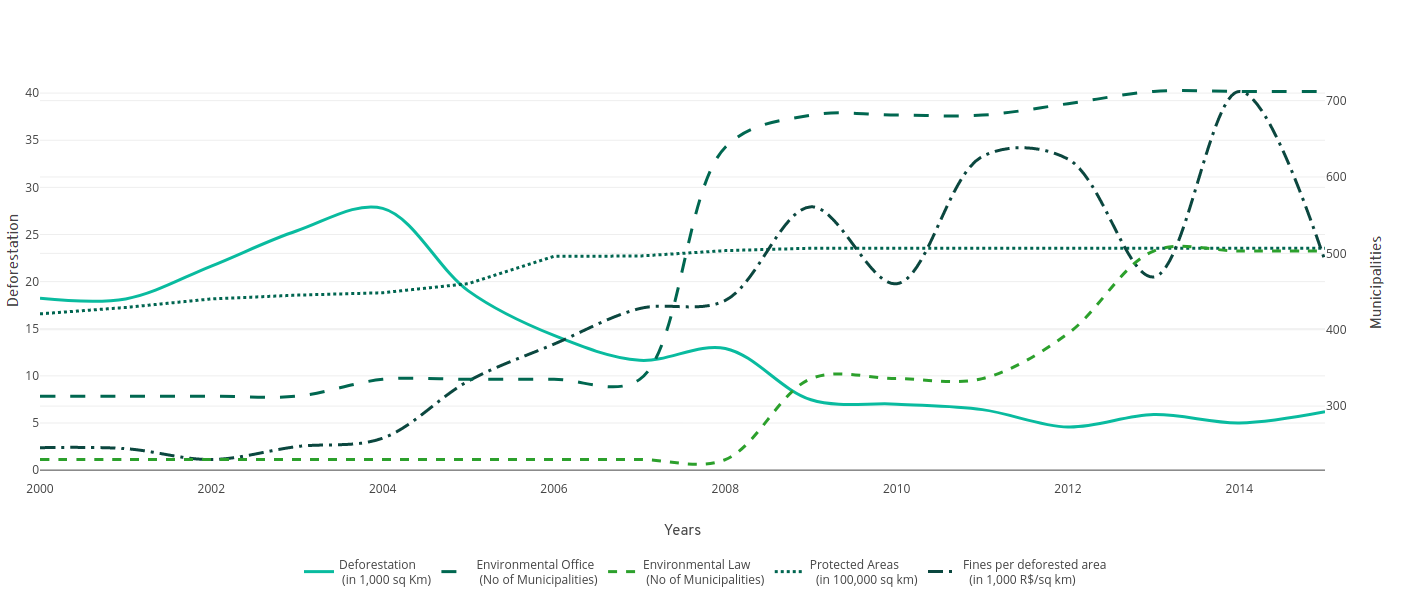
\includegraphics[width=1\linewidth, inner]{Figure1_policy_plot.png}
\caption{Deforestation in the Legal Amazon, Environmental Policy and the Institutional Environmental Framework (2004-2015). Source: \citep{inpe, MMMAwebsite, IBAMAwebsite}}
\label{fig:2}
\end{figure}

\begin{center}
\begin{figure}[ht]
  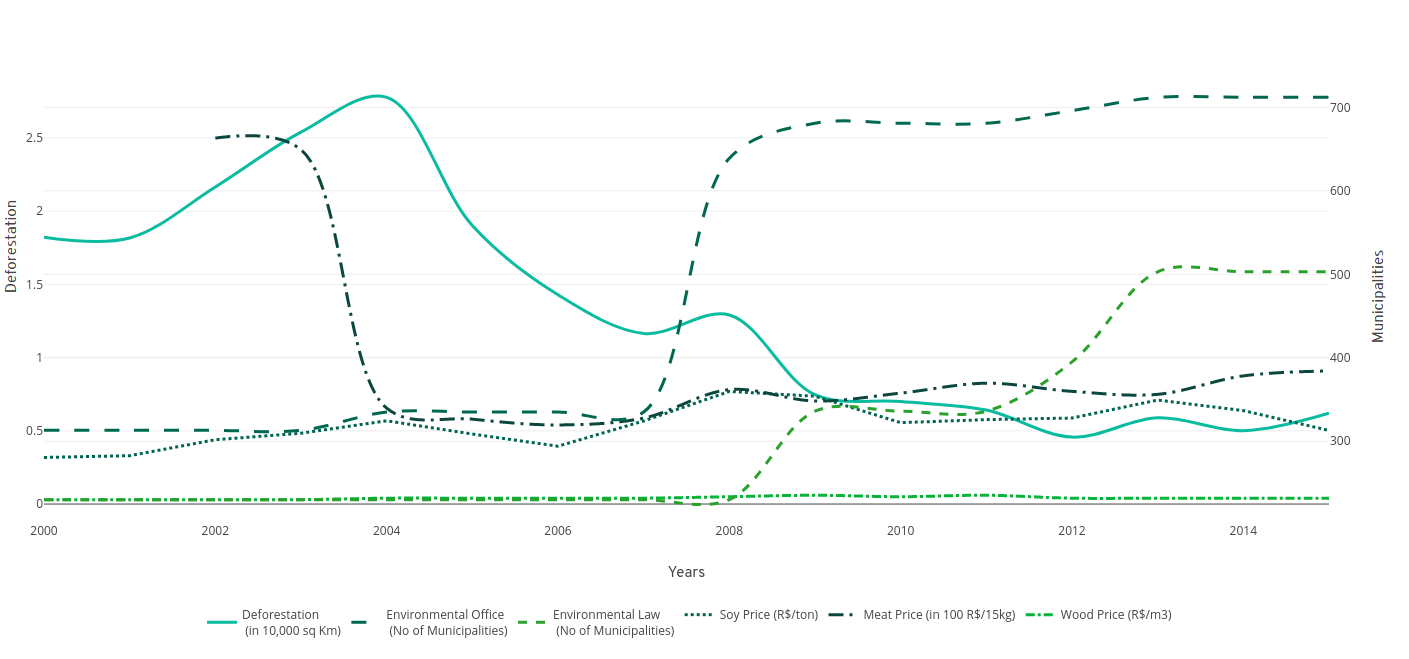
\includegraphics[width=1\linewidth]{Figure1_price_plot.png}
\caption{Deforestation in the Legal Amazon and commodities price the Institutional Environmental Framework (2004-2015). Source: \citep{inpe, IBGE1,CEPEA}}
\label{fig:3}
\end{figure}
\end{center}
\end{landscape}

%We calculate the intensity of the activity of the environmental police using the real value of fines issued within a municipality divided by deforestation in any given year (see \citet{hargrave_kis-katos_2012}).

\subsection{Empirical strategy}

In order to analyse the impact of different economic and environmental policies and commodity prices under different institutional settings our estimations are based on a panel of municipality level data between 2004 and 2015 which allows us to control for variability across municipalities.  Our baseline regression is given by:

\begin{equation}
    \text{ln}D_{i,t} = \mu_{i} + \text{X}_{i,t-1}\beta_{1}  + \text{X}_{i,t} \beta_{2} + \lambda_{t} + \varepsilon_{i,t} \label{eq:1} \\\\
\end{equation}


where the dependent variable, $lnD_{i,t}$, is the natural log of yearly deforestation in municipality \textit{i} in year \textit{t}. In addition, it includes a fixed parameter of time dummies that capture the effects of overall changes in the explanatory variables in deforestation, $\lambda_{t}$. The vector of controls, $X_{i,t-1}$, includes economic activity (GDP), agricultural prices at municipality level (Soy Price and Wood Price) and state level (Beef Price), access to markets (Roads), the number of settlements within each municipality (Settlements) and number of families per size of settlement (Settlement Density), the total amount of rural credits granted to recipients in a given municipality (Rural Credits) and an indicator variable for the existence of housing projects (Housing Projects) within a municipality, dummy variables to control for political factors (Mayor political party, Mayor education, Mayor gender, Mayor Age), the amount of commissioned workers standardised by population at municipality level (Corruption), and whether the mayor is re-elected or not (Re-election). Our policy variables include fines per municipality in any given year (Fines), the sum of the area of conservational units plus indigenous land per municipality level (Protected Areas). Finally, we include dummy variables for when a municipality has in place either an environmental law and environmental office (with a value of 1 from the year it was in place and zero otherwise.). Finally, we include cloud cover (Clouds) and not observed areas (No obs), $\text{X}_{i,t} \beta_{2}$.

As we are dealing with grouped data, the errors are inter-related and hence we include \citet{DRISCOLL} standard errors that are robust to autocorrelation, heteroskedasticity and cross-sectional dependence. The year and municipality level dummies are included to capture time and municipality invariant effects (e.g. climate, infrastructure or population).

In terms of our right hand side variables in $X_{i,t-1}$, one can conjecture a number of ex-ante expectations of their role in deforestation.  The commodity prices of beef, soy and wood are included to capture the influence of market conditions. For example, if the prices of beef and soy increase, there may be pressure for further deforestation to clear land for cultivation or grazing.  In the case of the price of wood, the effect is ambiguous as on the one hand, as prices rise it may lead to a greater incentive to harvest the forest.  On the other hand, higher prices may lead to a greater awareness of the value of forests and lead to greater efforts to protect what is now a more valuable resource. 
%Another hypothesis bases on the fact that much of Legal Amazon is wood-intensive fuel and increases in the demand for fuel, driven by income growth, induces forest growth as argued by \citet{FOSTER_2003}. 
It is worth to explain that much of deforestation is through illegal logging which we try to capture through market prices. In order to capture access to markets, we include the length of new federal roads and we believe it pressures to further deforestation the more roads and highways are constructed.

Turning to the environmental policies, the expectation is that each policy increases risk of being caught or the cost of transgressing an environmental law which should reduce expected profits associated with deforestation. Hence, we expect a negative sign on the coefficient from our environmental fines variable. The expected sign on our protected areas variable is ambiguous.  On the one hand, if an area is protected in more than name only with additional patrols for example, this should reduce the area in a municipality that can be easily deforested.  On the other hand, the decision to designate an area as protected may have been in response to previous deforestation  as noted by \citet{hargrave_kis-katos_2012} and may capture that deforestation problems are more severe in that particular area. The result of the introduction of a PA might simply be to shift the deforestation activities to areas just outside of the PA but still within a given municipality boundary \citep{GIRARDI}.\footnote{According to \citet{ICMBIO} and \citet{FUNAI} the signalling process of a PA is through signboards. These signboards are implanted in strategic places, that allow to guide the citizen on the access to that area or the transit in the same. Materialising their limits through fences, would have a high cost, which are beyond the resources available for the budget execution of demarcation / georeferencing. There are necessary protection procedures (for herds / planting areas or other protection needs) when requested by the community, but this happens in isolated and specific cases and it is not part of the delimitation of protected areas specifying their physical limits.}

In terms of other public policies we expect housing projects to have a negative impact on deforestation as the provision of affordable housing to inhabitants should reduce the incentive for agents to move to the frontier and clear forest for a place to live. The sign and significance of rural credit variable is uncertain. On the one hand, the availability of official subsidised credit may fuel deforestation by helping to fund clearing through investment in machinery, tools and fertilizers. On the other hand, if credit enables the development of a functioning market in forestry products it may improve forest management practices and reduce deforestation pressures. For our settlement variables, we expect that the number and density of settlements to result in an increase in the demand for deforestation although we expect this relationship to be non-linear hence we include squared terms of each variable.

Finally, our controls for environmental factors which are cloud cover and unobserved areas are expected to have positive and negative coefficients respectively. For unobserved areas, we expect that the greater the area not observed within a municipality, the more difficult it will be to detect the deforestation process. As for cloud cover, the hypothesis is that agents are aware of the policy monitoring program that employs satellite surveillance and may use cloudy days as a cover for their deforesting actions as the satellite may not detect their activity and hence it will reduce their chance of being caught and fined.  Hence, the more cloudy days recorded in a given year is expected to be a positive determinant of deforestation within that year.


%The within transformation removes the fixed municipality-specific effect $\mu_{i}$ and all variables are transformed as deviations from their municipality means. First, we take the average of equation \eqref{eq:1} over time and this gives


%\begin{equation}
%    \text{ln}\overline{D}_{i.} = \mu_{i} + \overline{\text{X}}_{i.}\beta  + \lambda_{t} + %\overline{{\varepsilon}_{i}}  \label{eq:2}
%\end{equation}
						

%Therefore, subtracts the equation \eqref{eq:2} from equation \eqref{eq:1} gives


%\begin{equation}
%	\text{ln}{D}_{i,t} - \text{ln}\overline{D}_{i.} = \beta({\text{X}_{i,t} - \overline{\text{X}}_{i.}}) + %(\varepsilon_{i,t} -  \overline{\varepsilon}_{i.})  \label{eq:3}
%\end{equation}

%Also, averaging across all municipalities in \eqref{eq:1} gives

%\begin{equation}
%    \text{ln}\overline{D}_{..} = \overline{\text{X}}_{..}\beta  + \overline{\varepsilon}_{..}  \label{eq:4}
%\end{equation}
	
%where we already assumed the restriction that the $\sum_{i=1}^{N} \mu_{i} $ = 0  and $\sum_{i=1}^{N} \lambda_{t} $ = 0. This is an arbitrary restriction on the dummy variable coefficients to avoid multicollinearity. In this case, $\widetilde{\beta}$ is obtained from regression \eqref{eq:4}, and the specific effect of each municipality ($\mu_{i}$) and the trend effect ($\lambda_{t}$) can be recovered from

%\begin{equation}
%\widetilde{\mu_{i}} = (\text{ln}\overline{D}_{i.} - \text{ln}\overline{D}_{..}) - %\widetilde{\beta}(\overline{X}_{i.} - \overline{X}_{..}) \label{eq:5}
%\end{equation}

%\begin{equation}
%\widetilde{\lambda_{t}} = (\text{ln}\overline{D}_{.t} - \text{ln}\overline{D}_{..}) - %\widetilde{\beta}(\overline{X}_{.t} - \overline{X}_{..}) \label{eq:6}
%\end{equation}



One of the main contributions of this study is to investigate the interaction between environmental institutions and environmental policies whilst taking into account the expansion in commodity markets captured through commodity prices of beef, wood and soy. Hence, we estimate \eqref{eq:1} given by:





\begin{equation}
\begin{gathered}
\text{ln}D_{i,t} = \mu_{i} + \text{X}_{i,t}\beta_{1} + \text{X}_{i,t-1}\beta_{2}  + \text{(IEF * Env. Policies)}_{i,t-1} \beta_{3} + \\ \text{(IEF * Prices)}_{i,t-1}  \beta_{4} + \lambda_{t} + \varepsilon_{i,t} \label{eq:2} 
\end{gathered}
\end{equation}



so we are able to estimate the extent to which the effectiveness of environmental policies depends on the institutional environmental framework that operates within a municipality. The expectation is that one would observe a reduction in those municipalities that have policies in place that are backed up by proper enforcement of the law through a well functioning institutional framework.  Likewise, in those municipalities the institutional framework is weak then environmental policies may not be introduced, pushed or enforced which would mean an insignificant or even positive effect on overall deforestation rates if loggers are attracted to or pushed from well regulated municipalities. Likewise, combining the institutional environmental framework within a municipality with growth in demand for commodities captured through commodities prices may lead to similar results. One possible driver of the implementation and enforcement of environmental policies are the characteristics and behaviour of the mayor who is in charge of a given municipality. Although we have no priors on age and gender we might expect education to have a negative influence of deforestation while we might expect a mayor that supports pro-farmer policies to have a positive influence on deforestation. The governance attitude of the politicians  within a municipality leading to a corrupted behaviour also has a positive impact on deforestation. Finally, it has been proved that mayors running for re-election tend to explore forests for economic reasons as a way of getting more votes.

One concern with regard to estimating equation \ref{eq:1} and equation \ref{eq:2} is the potential endogeneity of many of the explanatory variables, and hence their interpretation in terms of causality.  Since it would be difficult to find plausible instruments for many, if not for all, of our independent variables, we instead take a three pronged approach to alleviate any such concerns.  First, we control for municipality fixed effects, allowing us to purge all time invariant observables unobservables from the specifications.  Secondly, using an extensive set of other controls, as listed above, we hope to capture all likely determinants of deforestation.  Finally, we lag all control variables by one period, so that under assumption that, after controlling for fixed effects all confounding shocks are only contemporaneous in nature, we are left with solely exogenous variation in the elements of $X_{i,t-1}$.
%COLOCAR AQUI SOBRE IGNORAR ENDOGENEIDADE!!!

%********************************** % Fourth Section  *************************************

\section{Results}
\label{S:4}

\subsection{The effect of environmental policies and market expansion on deforestation}

Results from our estimation of equation \ref{eq:1} are presented in Table \ref{tab:results1}. Our baseline model includes 562 municipalities of the Legal Amazon. In columns (1) through (7) we experiment with including separately environmental policies, such as fines and protected areas, the prices of soy, wood and beef, and our institutional environmental framework variables given by our environmental law and environmental office dummies. Taking our institutional variables first (dummies for an environmental office and an environmental law) we find that neither is significant when included separately in Columns (3) or (4) or together in Column (8). This suggests that having an office and an environmental law in place is necessary but not sufficient to reduce deforestation.

Turning to our other controls, in Column (8) we include all the variables together, our preferred specification.  One immediate observation from Column(8) is that our fines variable is not a significant determinant of deforestation despite the rapid growth in fines levied during this period. One explanation is a lack of enforcement. The environmental police often have limited financial and manpower resources to issue fines but also insufficient legal means for collecting the fines once they have been issued no other way to collect the fine \citep{araujo_barreto_baima_gomes_2017}.  For the PA variable we find an increase in one unit of protected areas (10,000 km$^{2}$) is, ceteris paribus, associated with an increase of 2.7\% in deforestation the following year. To put this number into context we use the mean value of deforestation for our sample (20.2 km$^{2}$) and find out that this percentage would mean average increases in deforestation of 0.55 km$^{2}$.\footnote{It is important to stress that these calculations are only approximations to get an impression about the magnitude of the effect.} One explanation is that PAs are established in response to previous deforestation pressure which is then displaced to neighbouring areas just outside the PAs and is therefore capturing the presence of active groups of loggers in a municipality. In addition, this result might be related to the fact that there are potentially limited public monitoring and enforcement specially in sustainable use PAs in which certain economic activities are allowed \citep{RICO_2017}.\footnote{\citet{RICO_2017} also found a positive result to this relationship when analysing dynamics of forest loss and governance in PA's in the Peruvian Amazon.}

For our market demand variables we find that the estimated coefficient in Column (8) for the price of wood is significant and negative. All other variables remaining constant, an increase in wood price by one unit (1 BRL) leads to an average decrease in deforestation of 128\%. In terms of our sample, this percentage would mean average decreases in deforestation of approximately 26km$^{2}$. The coefficients on the price of beef and soy are not significant either together or individually.

In terms of our other economic policy variables, we find that the greater the number of settlements within a municipality the greater the degree of deforestation (a positive liner term) but at a decreasing rate (a negative squared term). Increasing the number of settlements will lead to, ceteris paribus, an increase in deforestation by nearly 6\%. The turning point is inside the sample range. We estimate the turning point to be 16 settlements within a municipality and from our sample we know that only five percent of our municipalities sample have passed the turning point which suggests that for the vast majority of municipalities additional settlements lead to increased deforestation.\footnote{Concei\c{c}\~{a}o do Araguaia - Par\'{a}, Itupiranga - Par\'{a}, Marab\'{a} - Par\'{a}, Novo Repartimento - Par\'{a} and Z\'{e} Doca - Maranh\~{a}o represent the municipalities with the highest number of settlements.} 

For our settlement density variable we find that increasing density settlements within a municipality leads to higher deforestation but that the effect is non-linear so that deforestation increases but at a decreasing rate. More densely populated settlements deforest more within a municipality as pressure on land and the need for expansion is greater. The high density turning point which is 0.62 includes only one settlement called Altamira in Para and is more developed economically leading to less pressure to deforest for economic purposes. Increasing the number of families per settlement within a municipality is associated with increasing deforestation at a decreasing rate of 280\%. Likewise, housing projects have a negative effect on deforestation as expected, since reduces the incentive for agents living in poor quality housing clear land to live. The estimated coefficient implies that the existence of housing projects within a municipality decreases logged deforestation by 15\%. To put this number into context, we use the mean value of deforestation for our sample (20.2 km$^{2}$) and detect that represents average decreases in deforestation of 3 km$^{2}$.

Turning to the political factors, we notice that only mayor age and corruption have a significant effect on deforestation. We find that an increase in age above the average (50 years) results in an average decrease in deforestation of 5.6$\%$. At the mean value of deforestation for our sample, we understand that this small fraction would represent an average decrease in deforested areas of 1.1km$^{2}$. The justification relies on the argument that younger politicians that want to stay in power for longer periods are more prone to undertake incentives that contradict the environmental agenda, while older politicians tend to be more experienced and cautious in dealing with environmental agendas. Corruption, mirrored in the number of commissioned workers per population, leads to higher deforestation within a municipality. In essence, an increase in number of commissioned workers per population by one unit  is associated with an increase of 2.4\% in deforestation. For our sample, this would represent an increase of 0.48 km$^{2}$ per each additional commissioned worker averaged by population. It is of interest to observe that corruption is positive and significant in columns (1) through (8), which endorses the necessity of this political control. Gender, being a pro-farmer politician, and having an education level of tertiary of above have no effect on deforestation rates.

\begin{table}[htp!]
\caption{Effects of Environmental Policies and Commodities Prices on Deforestation}
\scriptsize
       \begin{tabularx}{\columnwidth}{Z E E E E E E E E }
       \hline
     \hline
      Sample & \multicolumn{5}{l}{Dependent: $\Delta$ \textit{ln} Deforestation} \\ \cline{2-9}
      & (1) & (2) & (3) & (4) & (5) & (6) & (7) & (8) \\
        \hline
    Sett$_{-1}$ & 0.080***	&	0.070***	&	0.078***	&	0.079***	&	0.074***	&	0.079***	&	0.078***	&	0.064***\\
	                   & 	(5.36)	&	(4.59)	&	(5.61)	&	(5.50)	&	(4.87)	&	(5.50)	&	(5.08)	&	(3.98)	\\
    Sett$_{-1}$ sq & -0.002**	& -0.002**	& -0.002***	& -0.002***	&	-0.002**	&	-0.002**	&	-0.002**	&	-0.002**	\\
                        & 			(3.04)	&	(2.90)	&	(3.16)	&	(3.18)	&	(2.97)	&	(2.94)	&	(3.08)	&	(2.48)	\\
    Sett Dens$_{-1}$ & 4.056**	&	4.510***	&	4.159**	&	4.120**	&	3.866**	&	4.397***	&	4.116**	&	4.685***	\\
                        & 		(2.99)	&	(3.36)	&	(2.89)	&	(2.97)	&	(2.97)	&	(3.13)	&	(2.92)	&	(3.73)	\\
    Sett Dens$_{-1}$ sq & -3.639***	&	-3.212**	&	-3.620***	&	-3.581***	&	-3.283***	&	-3.841***	&	-3.581***	&	-3.353***	\\
                        & 	(3.51)	&	(2.88)	&	(3.41)	&	(3.50)	&	(3.60)	&	(3.70)	&	(3.47)	&	(3.34)	\\
    Rural Credits$_{-1}$ & 0.025	&	0.025*	&	0.024	&	0.024	&	0.024	&	0.024	&	0.028	&	0.028	\\
                        & 		(1.75)	&	(1.81)	&	(1.77)	&	(1.77)	&	(1.71)	&	(1.67)	&	(1.61)	&	(1.51)	\\
    Housing Projects$_{-1}$ & -0.147**	&	-0.150**	&	-0.147**	&	-0.147**	&	-0.150**	&	-0.147**	&	-0.149**	&	-0.153**	\\
                        & 		(2.92)	&	(2.83)	&	(2.91)	&	(2.92)	&	(2.91)	&	(2.93)	&	(2.80)	&	(2.71)	\\
    GDP$_{-1}$ & -0.237	&	-0.249	&	-0.234	&	-0.248	&	-0.232	&	-0.261	&	-0.232	&	-0.274	\\
                        & 	(1.50)	&	(1.56)	&	(1.46)	&	(1.53)	&	(1.50)	&	(1.60)	&	(1.52)	&	(1.66)	\\
    GDP$_{-1}$ sq & 0.027	&	0.028	&	0.027	&	0.027	&	0.025	&	0.031	&	0.026	&	0.031	\\
                        & 		(1.48)	&	(1.51)	&	(1.46)	&	(1.49)	&	(1.48)	&	(1.68)	&	(1.51)	&	(1.74)	\\
    Mayor Party$_{-1}$ & 0.041	&	0.039	&	0.039	&	0.042	&	0.037	&	0.039	&	0.042	&	0.036	\\
                        & 		(0.90)	&	(0.86)	&	(0.86)	&	(0.93)	&	(0.85)	&	(0.87)	&	(0.89)	&	(0.81)	\\
    Mayor Education$_{-1}$ &	0.010	&	0.016	&	0.011	&	0.011	&	0.012	&	0.019	&	0.011	&	0.024	\\
                        & 		(0.31)	&	(0.57)	&	(0.35)	&	(0.38)	&	(0.41)	&	(0.68)	&	(0.38)	&	(0.96)	\\
    Mayor Age$_{-1}$ & -0.065**	&	-0.062**	&	-0.063**	&	-0.064**	&	-0.060**	&	-0.062**	&	-0.060**	&	-0.056**	\\
                        & 		(2.46)	&	(2.38)	&	(2.40)	&	(2.46)	&	(2.41)	&	(2.29)	&	(2.61)	&	(2.39)	\\
    Mayor Gender$_{-1}$ &	0.025	&	0.025	&	0.023	&	0.021	&	0.020	&	0.030	&	0.022	&	0.030	\\
                        & 		(0.69)	&	(0.66)	&	(0.61)	&	(0.55)	&	(0.53)	&	(0.79)	&	(0.58)	&	(0.78)	\\
    Corruption$_{-1}$ & 0.026**	&	0.026**	&	0.026**	&	0.025**	&	0.026**	&	0.026**	&	0.025**	&	0.024**	\\
                        & 		(2.94)	&	(2.98)	&	(2.78)	&	(2.78)	&	(2.85)	&	(2.88)	&	(2.70)	&	(2.90)	\\
    Re-election$_{-1}$ &	0.004	&	0.002	&	0.003	&	0.003	&	-0.004	&	0.003	&	-0.000	&	-0.008	\\
    	                & (0.17)	&	(0.11)	&	(0.14)	&	(0.14)	&	(0.21)	&	(0.11)	&	(0.01)	&	(0.35)	\\
    Roads$_{-1}$ & -0.614	&	1.218	&	-0.954	&	-0.697	&	1.134	&	-0.646	&	-5.817	&	-2.007	\\
                        &  	(0.08)	&	(0.15)	&	(0.12)	&	(0.09)	&	(0.17)	&	(0.08)	&	(0.34)	&	(0.15)	\\              
    Clouds & 0.001	&	0.000	&	0.001	&	0.001	&	0.001	&	0.001	&	0.001	&	0.000	\\
                        & 	(0.61)	&	(0.47)	&	(0.60)	&	(0.59)	&	(0.63)	&	(0.59)	&	(0.61)	&	(0.47)	\\
    NoObs & 	-0.004	&	-0.002	&	-0.004	&	-0.003	&	-0.003	&	-0.003	&	-0.003	&	0.000	\\
                      	& (0.47)	&	(0.25)	&	(0.50)	&	(0.42)	&	(0.37)	&	(0.41)	&	(0.42)	&	(0.09)	\\
    Fines$_{-1}$ & 	-0.015	&		&		&		&		&		&		&	-0.018	\\
                        & 		(0.73)	&		&		&		&		&		&		&	(0.83)	\\
    PAs$_{-1}$ & 		&	0.027***	&		&		&		&		&		&	0.027***	\\
                        &  &	(4.10)	&		&		&		&		&		&	(3.89)	\\
    Env. Law$_{-1}$ & 		&		&	0.022	&		&		&		&		&	0.022	\\
                        & 			&		&	(0.95)	&		&		&		&		&	(1.00)	\\
    Env. Office$_{-1}$ &		&		&		&	-0.054	&		&		&		&	-0.058	\\
                        & 			&		&		&	(1.55)	&		&		&		&	(1.51)	\\
    Soy Price$_{-1}$  & 	&		&		&		&	0.630	&		&		&	0.549	\\
                        & 			&		&		&		&	(1.27)	&		&		&	(1.18)	\\
    Wood Price$_{-1}$  & 	&		&		&		&		&	-1.331*	&		&	-1.285*	\\
                        & 		&		&		&		&		&	(2.02)	&		&	(2.11)	\\
    Beef Price$_{-1}$  & 		&		&		&		&		&		&	1.664	&	1.180	\\
                        & 		&		&		&		&		&		&	(0.58)	&	(0.49)	\\
    \hline
    %Other Set of Controls &  Yes & Yes & Yes & Yes \\
    Year Fixed Effects &   Yes & Yes & Yes & Yes & Yes & Yes & Yes & Yes \\
    Municipality Fixed Effects &   Yes & Yes & Yes & Yes & Yes & Yes & Yes & Yes \\
    Number of Observations &   6,178 &   6,178 &   6,178 &   6,178 &   6,178 &   6,178 &   6,178 &   6,178\\
    \hline 
    \hline
    \multicolumn{9}{l}{*, **, *** denote significance at 10$\%$, 5$\%$ and 1$\%$ levels, respectively. Robust standard error values are }\\
    \multicolumn{9}{l}{indicated in parentheses under the coefficients.  PAs stand for Protected Areas.}\\
\end{tabularx}
\label{tab:results1}
\end{table}

\subsection{Environmental policies and market expansion conditioning on institutional environmental framework}
\label{SS:4.1}

In Table \ref{tab:results2} we consider the impact of our policy variables and commodities prices conditional on the institutional environmental framework with the same set of controls from Table \ref{tab:results1} and the year fixed effects (Columns 1-8). In Column 9 we show that agents from municipalities that receive fines when there is an environmental law in place does not reduce deforestation. One explanation is that in the Legal Amazon many local environmental laws are not enforced following environmental incidents even though the municipalities have the power to do so. Thus, it seems more likely that the offender will be punished at the state or federal level rather than at the municipality level, which contributes to the limited effectiveness of fines as a punitive instrument at the local level.

In contrast, we find that there is a significant drop in deforestation through a policy of fines if an environmental office exists. More specifically, the estimated average drop in deforestation associated with the fines policy when there is a municipality with an environmental office is around 1.8 km$^{2}$ ceteris paribus. This finding illustrates that the coordinated process of implementation of the national environmental system (SISNAMA) that decentralises forces to assist the protection of the environment can have a positive effect curbing deforestation. Environmental offices appear to act as a primary partner to the SISNAMA together with IBAMA, which operates at the national level as an administrative arm and environmental police of the Brazilian Ministry of Environment. This coalition appears to make the institutional framework work more effectively at the local level. 

We also find that municipalities with an environmental office and protected areas within their territory tend to increase deforestation by approximately 3\%. Using the mean value of deforestation for our sample (20.2 km$^{2}$) we detect that this percentage represents average increases in deforestation of 0.6 km$^{2}$. This unexpected result may be because environmental offices are often set up to work together with other offices, such as agriculture, tourism, education, and infrastructure offices. In this sense environmental management is often associated with other themes and the creation of joint offices can lead to conflict with the agendas of others. For example, given that expansion of agriculture is an important factor in deforestation, having a joint office of environment and agriculture could lead to a conflict of interest. Regarding protected areas, conditioned on environmental laws at the municipality level, we find no significant effect.  This suggests that protected areas are not entirely monitored at the local level since a substantial number of these units are regulated at the state and federal level. 

Turning to our commodity market variables, we find that the institutional environmental framework plays an important role when conditioned on commodity prices. Soy prices conditioned on the existence of environmental law correspond to averages decreases of deforestation of almost 73\%. Arguably much of this effect is likely to be the result of the moratorium implemented in 2006.\footnote{The moratorium establishes that companies purchasing the grain and its derivatives can not acquire from those who produced in deforested areas after 2008, within indigenous lands or that are on the slave labour list. The moratorium instrument prohibited soy producers from negotiating the sale of production originating from deforested areas in the legal Amazon for a period of two years.}  In this sense, the institutional environmental framework was used to help compliance with the soy moratorium. However, when looking to the overall effect we can observe that soy price influence deforestation positively. An increase in soy price by one unit (1 BRL) at mean values for the existence of environmental law is, ceteris paribus, associated with an average increase in deforestation of approximately 46\%. We find no significant effect for other commodities when conditioning on the existence of an environmental law. \footnote{Recently, \citet{CAVIGLIAHARRIS2018232} addressed the existence of a nonlinear relationship with the intensification of cattle production in part of the Legal Amazon. First as farms become more intensive the demand for newly cleared land increases, but then decreases with further intensification.}

In contrast, wood (negative) and beef (positive) prices are significant when conditioned on environmental office. This is consistent with our assumptions that environmental management offices are associated with other strategic themes and that a institutional framework on its own fails to protect the environment. From our sample, forestry prices have a negative impact on deforestation and beef market has a positive impact on deforestation. Taking the mean value of deforestation (20.2 km$^{2}$) we find out that forestry prices would produce average decreases in deforestation of 38 km$^{2}$ and for the beef market we would see average increases in deforestation of 1.4 km$^{2}$.

\begin{landscape}
\begin{table}[htpb!]
\caption{Effects of Environmental Policies on Deforestation: Baseline Model}
\scriptsize
\begin{tabularx}{0.82\linewidth}{l Z Z Z Z Z Z Z Z Z}
     \hline
     \hline
      Sample & \multicolumn{9}{l}{Dependent: $\Delta$ \textit{ln} Deforestation} \\ \cline{2-10}
      & (1) & (2) & (3) & (4) & (5) & (6) & (7) & (8) & (9) \\
        \hline
        
    %%%%%%%%%%%%%%%%%%%%%%%%%%%%%%%%%%%%%%%%%%%%%%%%%%%%%%%%%%%%%%%%%%%%%%%%
    %%%%%%%%%%%%%%%%%%%%%%%%%%%%%%%%%%%%%%%%%%%%%%%%%%%%%%%%%%%%%%%%%%%%%%%%
    %%%%%%%%%%%%%FALTA ATUALIZAR OS DADOS EM VERDE%%%%%%%%%%%%%%%%%%%%%%%%%%
    %%%%%%%%%%%%%%%%%%%%%%%%%%%%%%%%%%%%%%%%%%%%%%%%%%%%%%%%%%%%%%%%%%%%%%%%
    %%%%%%%%%%%%%%%%%%%%%%%%%%%%%%%%%%%%%%%%%%%%%%%%%%%%%%%%%%%%%%%%%%%%%%%%
    
    %Settlements$_{-1}$ & 0.064***	&	0.060***	&	0.063***	&	0.065***	&	0.064***	&	0.060*** &	0.061***&	0.063***	&	0.062***\\
    %                    & 	(3.71)	&	(3.66)	&	(4.12)	&	(4.17)	&	(3.99)	&	(3.48)	&	(3.64)	&	(3.86)	&	(3.79)\\
    %Settlements$_{-1}$ sq & -0.001*	&	-0.001*	&	-0.001**	&	-0.001*	&	-0.001**	&	-0.001*	&	-0.001*	&	-0.001*	&	-0.001**\\
    %                    & 		(2.05)	&	(2.10)	&	(2.21)	&	(2.17)	&	(2.21)	&	(2.00)	&	(2.04)	&	(2.04)	&	(2.01)\\
    %Settlements Dens$_{-1}$ & 4.568***	&	4.653***	&	4.583***	&	4.765***	&	4.511*** &	4.640*** &	4.640*** &	4.806***	&	4.772***\\
    %                    & 	(3.76)	&	(3.94)	&	(3.72)	&	(3.93)	&	(3.66)	&	(3.97)	&	(3.95)	&	(4.11)	&	(4.09)\\
    %Settlements Dens$_{-1}$ sq & -3.712***	&	-3.639***	&	-3.694***	&	-3.820*** &	-3.653*** &	-3.667*** &	-3.673*** &	-3.790***	&	-3.769***\\
    %                    & 	(3.96)	&	(4.16)	&	(3.84)	&	(4.11)	&	(3.86)	&	(4.24)	&	(4.18)	&	(4.32)	&	(4.30)\\
    %Rural Credits$_{-1}$ & 1.948	&	1.589	&	1.587	&	1.823	&	1.732	&	1.803	&	1.642	&	1.672	&	1.664\\
    %                    & 	(1.31)	&	(1.07)	&	(1.08)	&	(1.21)	&	(1.13)	&	(1.25)	&	(1.16)	&	(1.20)	&	(1.20)\\
    %Housing Projects$_{-1}$ & -0.142**	& -0.147** &	-0.138**	&	-0.133**	&	-0.143** & -0.146**	&	-0.141**	&	-0.131**	&	-0.131**\\
    %                    & 	(2.55)	&	(2.73)	&	(2.56)	&	(2.51)	&	(2.56)	&	(2.72)	&	(2.72)	&	(2.66)	&	(2.65)\\
    %GDP$_{-1}$ & -0.214	&	-0.231	&	-0.204	&	-0.225	&	-0.221	&	-0.230	&	-0.220	&	-0.229	&	-0.226\\
    %                   &  (1.43)	&	(1.53)	&	(1.23)	&	(1.57)	&	(1.46)	&	(1.51)	&	(1.29)	&	(1.38)	&	(1.39)\\
    %GDP$_{-1}$ sq & 0.026	&	0.027	&	0.026	&	0.028*	&	0.026	&	0.027	&	0.027	&	0.029	&	0.029\\
    %                    & 	(1.60)	&	(1.67)	&	(1.50)	&	(1.80)	&	(1.64)	&	(1.64)	&	(1.51)	&	(1.65)	&	(1.66)\\
    %Mayor Party$_{-1}$ & 0.042	&	0.040	&	0.048	&	0.041	&	0.045	&	0.038	&	0.043	&	0.042	&	0.042\\
    %                   & 	(0.95)	&	(0.92)	&	(1.09)	&	(0.94)	&	(1.03)	&	(0.88)	&	(0.97)	&	(0.95)	&	(0.95)\\
    %Mayor Education$_{-1}$ & 0.013	&	0.022	&	0.013	&	0.016	&	0.017	&	0.019	&	0.015	&	0.014	&	0.015\\
    %                    & 	(0.50)	&	(0.84)	&	(0.48)	&	(0.59)	&	(0.63)	&	(0.73)	&	(0.59)	&	(0.56)	&	(0.58)\\
    %Mayor Age$_{-1}$ & -0.060**	&	-0.057*	&	-0.058**	&	-0.059**	&	-0.060**	&	-0.056*	&	-0.053*	&	-0.053*	&	-0.052*\\
    %                   & 	(2.39)	&	(2.20)	&	(2.30)	&	(2.33)	&	(2.43)	&	(2.17)	&	(2.03)	&	(1.97)	&	(1.97)\\
    %Mayor Gender$_{-1}$ & 	0.026	&	0.027	&	0.029	&	0.029	&	0.031	&	0.024	&	0.023	&	0.024	&	0.024\\
    %                    & 	(0.65)	&	(0.68)	&	(0.71)	&	(0.72)	&	(0.78)	&	(0.60)	&	(0.59)	&	(0.60)	&	(0.61)\\
    %Corruption$_{-1}$ & 0.026***	&	0.026***	&	0.026***	&	0.025***	&	0.025**	&	0.026***	&	0.026*** & 0.026***	&	0.026***\\
    %                   & (3.26)	&	(3.22)	&	(3.76)	&	(3.19)	&	(3.10)	&	(3.35)	&	(4.02)	&	(4.07)	&	(4.06)\\
    %Roads$_{-1}$ & -0.106	&	0.971	&	2.265	&	2.292	&	-0.337	&	0.750	&	3.055	&	5.021	&	4.060\\
    %                   & 	(0.01)	&	(0.08)	&	(0.18)	&	(0.17)	&	(0.03)	&	(0.06)	&	(0.24)	&	(0.38)	&	(0.30)\\
    %Clouds$_{-1}$ & 0.013**	&	0.013**	&	0.014**	&	0.012**	&	0.013**	&	0.013**	&	0.013**	&	0.012**	&	0.012**\\
    %                    & 	(2.50)	&	(2.76)	&	(2.83)	&	(2.53)	&	(2.85)	&	(2.47)	&	(2.47)	&	(2.26)	&	(2.25)\\
    %Forest$_{-1}$ & 0.020*	&	0.022**	&	0.022**	&	0.019*	&	0.021**	&	0.020*	&	0.020*	&	0.018*	&	0.018*\\
    %                    & 	(2.19)	&	(2.48)	&	(2.53)	&	(2.19)	&	(2.55)	&	(2.18)	&	(2.18)	&	(1.96)	&	(1.95)\\
    Fines$_{-1}$ & 0.079	&	-0.019	&	-0.018	&	-0.017	&	-0.018	&	0.080*	&	0.083*	&	0.069	&	0.069	\\
                        & 	(1.73)	&	(0.89)	&	(0.84)	&	(0.80)	&	(0.84)	&	(1.82)	&	(1.90)	&	(1.64)	&	(1.62)	\\
    Protected Areas$_{-1}$ & 0.027***	&	-0.004	&	0.026***	&	0.026***	&	0.027***	&	-0.004	&	-0.005	&	-0.003	&	-0.003	\\
                        & 		(3.99)	&	(0.38)	&	(3.73)	&	(3.79)	&	(3.91)	&	(0.35)	&	(0.43)	&	(0.30)	&	(0.30)	\\
    Env. Law$_{-1}$ &	0.024	&	0.008	&	0.478***	&	0.079*	&	0.072*	&	0.010	&	0.470***	&	0.532***	&	0.538***	\\
                        & 	(1.04)	&	(0.36)	&	(3.38)	&	(2.12)	&	(2.19)	&	(0.39)	&	(3.27)	&	(3.18)	&	(3.22)	\\
    Env. Office$_{-1}$ & -0.041	&	-0.094*	&	0.122	&	0.131**	&	-0.101	&	-0.077	&	0.125	&	0.293	&	0.287	\\
                        & 	(1.03)	&	(2.06)	&	(0.63)	&	(2.38)	&	(1.27)	&	(1.61)	&	(0.63)	&	(1.45)	&	(1.45)	\\
    Soy Price$_{-1}$  & 0.551	&	0.558	&	1.068**	&	0.553	&	0.549	&	0.561	&	1.109***	&	1.114***	&	1.188**	\\
                        & 	(1.17)	&	(1.21)	&	(3.06)	&	(1.20)	&	(1.18)	&	(1.21)	&	(3.20)	&	(3.12)	&	(3.10)	\\
    Wood Price$_{-1}$  & -1.263*	&	-1.282*	&	-1.294*	&	0.855	&	-1.280*	&	-1.261*	&	-1.270*	&	0.686	&	0.639	\\
                        & 	(2.08)	&	(2.19)	&	(2.12)	&	(1.13)	&	(2.11)	&	(2.16)	&	(2.17)	&	(0.90)	&	(0.81)	\\
    Beef Price$_{-1}$  & 	1.089	&	1.109	&	1.232	&	0.791	&	1.200	&	1.014	&	1.060	&	0.723	&	0.685	\\
                        & 	(0.44)	&	(0.47)	&	(0.53)	&	(0.33)	&	(0.50)	&	(0.42)	&	(0.46)	&	(0.31)	&	(0.29)	\\
    Env. Law$_{-1}$* Fines$_{-1}$ & -0.009	&		&		&		&		&	-0.012	&	-0.014	&	-0.012	&	-0.012	\\
                        & 		(0.47)	&		&		&		&		&	(0.71)	&	(0.91)	&	(0.74)	&	(0.73)	\\
    Env. Office$_{-1}$* Fines$_{-1}$& -0.101**	&		&		&		&		&	-0.101***	&	-0.103***	&	-0.089**	&	-0.088**	\\
                        & (3.03)	&		&		&		&		&	(3.12)	&	(3.18)	&	(2.79)	&	(2.77)	\\
    Env. Law$_{-1}$* PAs$_{-1}$ &	&	0.007	&		&		&		&	0.008	&	0.008	&	0.007	&	0.007	\\
                        & 				&	(1.29)	&		&		&		&	(1.44)	&	(1.50)	&	(1.40)	&	(1.38)	\\
    Env. Office$_{-1}$* PAs$_{-1}$& 		&	0.029**	&		&		&		&	0.029**	&	0.029**	&	0.028**	&	0.028**	\\
                        & 		&	(2.95)	&		&		&		&	(2.94)	&	(2.93)	&	(2.82)	&	(2.83)	\\
    Env. Law$_{-1}$* Soy Price$_{-1}$  &  	&		&	-0.716***	&		&		&		&	-0.721***	&	-0.736***	&	-0.729***	\\
                        & 			&		&	(3.55)	&		&		&		&	(3.40)	&	(3.47)	&	(3.16)	\\
    Env. Office$_{-1}$* Soy Price$_{-1}$& 		&		&	-0.308	&		&		&		&	-0.346	&	-0.339	&	-0.447*	\\
                        &  			&					&	(1.09)	&		&		&		&	(1.21)	&	(1.25)	&	(1.90)	\\
    Env. Law$_{-1}$* Wood Price$_{-1}$&  	&		&		&	-0.483*	&		&		&		&	-0.442	&	-0.450	\\
                        &  				&		&		&	(2.19)	&		&		&		&	(1.65)	&	(1.69)	\\
    Env. Office$_{-1}$* Wood Price$_{-1}$ & 	&		&		&	-2.120***	&		&		&		&	-1.941***	&	-1.891***	\\
                        &  				&		&		&	(6.92)	&		&		&		&	(5.67)	&	(5.35)	\\
    Env. Law$_{-1}$* Beef Price$_{-1}$& 	&		&		&		&	-0.060**	&		&		&		&	-0.011	\\
                        &  				&		&		&		&	(2.54)	&		&		&		&	(0.50)	\\
    Env. Office$_{-1}$* Beef Price$_{-1}$ &		&		&		&		&	0.049	&		&		&		&	0.070**	\\
                        &  			&		&		&		&	(1.26)	&		&		&		&	(2.26)	\\
    \hline
    Set of Controls &   Yes & Yes & Yes & Yes & Yes & Yes & Yes & Yes & Yes \\
    Year Fixed Effects &   Yes & Yes & Yes & Yes & Yes & Yes & Yes & Yes & Yes \\
    Municipality Fixed Effects &   Yes & Yes & Yes & Yes & Yes & Yes & Yes & Yes & Yes \\
    Number of Observations &   6,178 &   6,178 &   6,178 &   6,178 &   6,178 &   6,178 &   6,178 &   6,178 &   6,178\\
    \hline
    \hline
    \multicolumn{10}{l}{ *, **, *** denote significance at 10$\%$, 5$\%$ and 1$\%$ levels, respectively. Robust standard error values are indicated in parentheses under the coefficients. PAs }\\
    \multicolumn{10}{l}{stand for Protected Areas.}\\
    \end{tabularx}%
  \label{tab:results2}%
\end{table}%
\end{landscape}

\subsection{Spatial Analysis}
\label{SS:4.2}

It is possible that deforestation has a spatial dependence i.e. deforestation process affects neighbouring municipalities and when there is a strong institutional environment there is a possibility to shift deforestation to municipalities with low enforcement. In order to check this assumption, we conduct a spatial analysis of spatial dependence following \citet{ANSELIN} and \citet{elhorst_2012}. The existence of spatial autocorrelation can occur if a given event in a given place has a significant impact on neighbouring regions. Spatial dependence relates to the idea of relative location and the interdependence between regions and the spillover effects of certain activities or factors and that interdependence may affect both the characteristics of the data and the nature of the events. Spatial econometric models with panel data capture the relationship between variables over time and arising for the existence for spatial autocorrelation. It should be added that it is assumed that the area studied remains constant over the period of years \citep{ALMEIDA}. 
For this analysis, we needed a strong balanced panel, so our sample reduced from 562 to 456 which is still represents 65\% of total Legal Amazon municipalities. We performed LM tests to establish the dependence factor (see Table \ref{tab:LMtests}). Up to this point, the test results pointed to the spatial lag model specification. In view of testing procedure we ran the two models, spatial auto-regressive model (SAR), spatial error model (SEM) (not shown here) and SAR is preferred to SEM in all specifications. 

To incorporate the autocorrelation of spatial lag type of dependent variable, our fixed effects model needs to be modified, generating the Spatial Autoregressive model with fixed effects:


\begin{equation}
\begin{gathered}
\text{ln}D_{i,t} = \mu_{i} + \rho W_{1}y_{t} +  \text{X}_{i,t}\beta_{1} + \text{X}_{i,t-1}\beta_{2}  + \text{(IEF * Env. Policies)}_{i,t-1} \beta_{3} + \\ \text{(IEF * Prices)}_{i,t-1}  \beta_{4} + \lambda_{t} + \varepsilon_{i,t} \label{eq:2} 
\end{gathered}
\end{equation}

where $W_{1}y_{t}$ is the spatial lag of the dependent variable. The spatial weight matrix W is defined according to various criteria and is maintained unchanged for all years of the panel. The calculation of the spatial weight matrices used the coordinates from the municipality's centroid. We calculated three different weight matrices. Our baseline weight matrix (W1) finds the 5 nearest neighbours and constructs a spatial weight matrix based on this number of neighbours, normalised to have row-sums of unity. Alternatively, we create a distance based spatial weight matrix (W2) with bands using latitude and longitude coordinates a the Great Circle distance formula. The bands used were 1km to 100km. Finally, we construct a distance based spatial weight matrix (W3) using latitude and longitude coordinates and the Great Circle distance formula (Lacombe's Method) \citep{elhorst_2012}. Using these techniques we gradually increase the number of neighbours.

Since it is not possible to compare the coefficient estimates in the non-spatial model, our baseline, with their counterparts in the spatial models SAR, we use the direct and indirect effects estimates as a result of impacts passing through neighbouring municipalities and back to the municipalities themselves. These feedback effects are partly due to the coefficient of the spatially lagged dependent variable. Within this perspective, we follow \cite{lesage_pace_2009} and present he direct, indirect and total effect of the coefficients separately.

Table \ref{tab:spatialW} report our results for the three different matrices. All results are consistent with the literature \citep{LAMBIN1, LAMBIN2}. We first consider the direct effect of our estimates. We can see that one of the institutional apparatus - environmental law - has no direct effect when conditioning on protected areas and, wood and beef commodities. Our spatial correlation is positive and significant and can be interpreted as the impact of changes in municipality on deforestation. The impact would be magnified by 1.2 and 1.6 through the spatial lag in the model. For our baseline weight matrix (W), we can see that the direct effect of Fines, from the SAR model, on deforestation was underestimated by a factor of 0.75. Since the direct effect of Fines is 0.517 and its coefficient estimate 0.596, its feedback effect
amounts to 0.07 or 15\% of the direct effect. In other words, these feedback effects turn out to be relatively reasonable. For environmental law and office using the second approach of weights we account that their effect amounts to 0.24 and 0.15 or 79\% and 14\% of the direct effect respectively. Looking to the indirect effect on the third model (W3), we can clearly see that the indirect effect of a change in the amount of fines issued appears to be 62\% of the direct effect. If the amount of fines issued increase in one municipality, the change in neighbouring municipalities to the change in the municipality itself is in the proportion of approximately 1 to 1.6 in case of increasing Fines. 

Overall, we can observe that the Institutional Environmental Framework (IEF) when established in a municipality tend to detain deforestation in neighbouring municipalities. As an example, in all of our specifications conditioning the existence of the IEF and the exercise of fines we have a negative effect on neighbouring municipalities. We can see the same effect for the market expansion conditioned on the IEF which corroborates with our main findings \ref{tab:results2}. 

\begin{table}[ht!]
\caption{Spatial Analysis - Baseline Model}
\footnotesize
       \begin{tabularx}{1\textwidth}{l XXX}
     \hline
     \hline
        \multicolumn{4}{l}{Dependent: $\Delta$ \textit{ln} Deforestation}\\ \cline{1-4}
    Sample & W1 & W2 & W3 \\
        \hline
    Fines$_{-1}$ &	0.596	(10.549) &	0.595 (10.532) &	0.599	(10.742)\\
    Protected Areas$_{-1}$ &	-0.025	(-1.891)&	-0.025 (-1.890) &	-0.030	(-2.281) \\
    Env. Law$_{-1}$ &	0.542	(2.369) &	0.543 (2.375) &	0.578	(2.560) \\
    Env. Office$_{-1}$&	1.193	(4.684) &	1.191 (4.677) &	1.221	(4.854)\\
    Soy Price$_{-1}$&	1.175	(3.080) & 1.174 (3.078)	 &	1.261	(3.348)\\
    Wood Price$_{-1}$&	4.429	(6.034) & 4.428 (6.032)& 	4.200	(5.794)	\\
    Beef Price$_{-1}$	&	1.963	(1.627) & 1.962 (1.626)& 1.752	(1.470)\\
    Env. Law$_{-1}$* Fines$_{-1}$	&	-0.174	(-5.164) & -0.174	(-5.152)&	-0.174	(-5.216)\\
    Env. Office$_{-1}$* Fines$_{-1}$&	-0.203	(-3.767) & -0.202	(-3.755)&	-0.213	(-4.015) 	\\
    Env. Law$_{-1}$* PAs$_{-1}$	&	-0.001	(-0.113) & -0.001	(-0.118)& 0.001	(0.163)\\
    Env.Office$_{-1}$*PAs$_{-1}$  &	0.014	(1.073) &	 0.014	(1.072)& 0.016	(1.264)\\
    Env. Law$_{-1}$* Soy Price$_{-1}$	&	-0.823	(-2.296) & -0.825	(-2.301)& 	-0.846	(-2.390) \\
    Env. Office$_{-1}$* Soy Price$_{-1}$&	-1.036	(-2.504) &		-1.035	(-2.500)& -1.094	(-2.676)\\
    Env. Law$_{-1}$* Wood Price$_{-1}$&	0.707	(1.317) &	0.708	(1.317)& 0.522	(0.984)\\
    Env. Office$_{-1}$* Wood Price$_{-1}$&	-2.442	(-3.171) & -2.440	(-3.168)& -2.350	(-3.089)  \\
    Env. Law$_{-1}$* Beef Price$_{-1}$&	-0.050	(-0.506) &	-0.050	(-0.507)&  -0.059	(-0.607) \\
    Env. Office$_{-1}$* Beef Price$_{-1}$&	-0.034	(-0.355) & -0.034	(-0.352)& -0.026	(-0.267) \\
    \sigma^{2} & 2.081 & 2.081 & 2.030  \\
    \rho & 0.168 (8.904) & 0.167 (8.847) & 0.389 (14.711)\\
    (Pseudo) R^{2} & 0.44 & 0.45 & 0.46 \\
    LogLik & -9541.60 & -9541.62 &  -9484.62   \\
    AIC & 19155 & 19155 & 19042  \\
    BIC & 19393 & 19393 &  19280 \\
    \hline
	\hline
    \multicolumn{4}{l}{t-values are indicated in parentheses next to the coefficients. PAs stands for Protected Areas.}\\
   \end{tabularx}%
  \label{tab:spatialW}%
\end{table}%


    \begin{table}[htpb!]
\caption{Spatial Analysis - Baseline Model - Effects}
\footnotesize
\centering
       \begin{tabularx}{0.8\textwidth}{l XXX}
     \hline
     \hline
        \multicolumn{4}{l}{Dependent: $\Delta$ \textit{ln} Deforestation}\\ 
        \hline
    Sample & W1 & W2 & W3 \\
        \hline
    \multicolumn{4}{c}{Direct Effects} \\ 
    \hline
    Fines$_{-1}$ & 0.599 (10.501) & 0.598 (10.485) & 0.603 (10.840)\\
    Protected Areas$_{-1}$& -0.024 (-1.800) & -0.024 (-1.800) & -0.030 (-2.292)\\
    Env. Law$_{-1}$ & 0.550 (2.386) & 0.552 (2.393) & 0.597 (2.633)\\
    Env. Office$_{-1}$ & 1.201 (4.612) & 1.200 (4.606) & 1.238 (4.881)\\
    Soy Price$_{-1}$ & 1.197 (3.150) & 1.196 (3.148) & 1.287 (3.381)\\
    Wood Price$_{-1}$ & 4.454 (6.036) & 4.453 (6.035) & 4.225 (6.012)\\
    Beef Price$_{-1}$ & 1.964 (1.594) & 1.964 (1.593) & 1.724 (1.398)\\
    Env. Law$_{-1}$* Fines$_{-1}$ & -0.173 (-5.157) & -0.173 (-5.161) & -0.174 (-5.179)\\
    Env. Office$_{-1}$* Fines$_{-1}$ & -0.205 (-3.784) & -0.205 (-3.773) & -0.214 (-3.924)\\
    Env. Law$_{-1}$* PAs$_{-1}$	& -0.001 (-0.115) & -0.001 (-0.121) & 0.001 (0.121)\\
    Env.Office$_{-1}$*PAs$_{-1}$ & 0.013 (1.011) & 0.014 (1.010) & 0.016 (1.253)\\
    Env. Law$_{-1}$* Soy Price$_{-1}$& -0.843 (-2.360) & -0.846 (-2.366) & -0.870 (-2.454)\\
    Env. Office$_{-1}$* Soy Price$_{-1}$ & -1.052 (-2.491) & -1.051 (-2.488) & -1.114 (-2.668)\\
    Env. Law$_{-1}$* Wood Price$_{-1}$ & 0.696 (1.304) & 0.696 (1.305) & 0.515 (0.968)\\
    Env. Office$_{-1}$* Wood Price$_{-1}$ & -2.422 (-3.091) & -2.420 (-3.088) & -2.350 (-3.183)\\
    Env. Law$_{-1}$* Beef Price$_{-1}$ & -0.045 (-0.458) & -0.046 (-0.459) & -0.059 (-0.619)\\
    Env. Office$_{-1}$* Beef Price$_{-1}$ & -0.032 (-0.324) & -0.032 (-0.322) & -0.026 (-0.277) \\
    \hline
    \multicolumn{4}{c}{Indirect Effects} \\ 
    \hline
    Fines$_{-1}$ & 0.119 (6.203) & 0.119 (6.180) & 0.375 (7.063)\\
    Protected Areas$_{-1}$ & -0.004 (-1.736) & -0.005  (-1.735) & -0.018 (-2.210)\\
    Env. Law$_{-1}$ &0.109 (2.282) & 0.109 (2.287) & 0.372 (2.520)\\
    Env. Office$_{-1}$ & 0.240 (3.866)& 0.238 (3.857) & 0.771 (4.234)\\
    Soy Price$_{-1}$ & 0.239 (2.862) & 0.237 (2.859) & 0.803 (3.121)\\
    Wood Price$_{-1}$ & 0.889 (4.675) & 0.884 (4.665) & 2.631 (4.955)\\
    Beef Price$_{-1}$& 0.393 (1.560) & 0.391 (1.559) & 1.070 (1.380)\\
    Env. Law$_{-1}$* Fines$_{-1}$& -0.034 (-4.281) & -0.034 (-4.268) & -0.108 (-4.584)\\
    Env. Office$_{-1}$* Fines$_{-1}$& -0.041 (-3.378) & -0.041 (-3.367) & -0.133 (-3.582)\\
    Env. Law$_{-1}$* PAs$_{-1}$	& -0.000 (-0.114)& 0.000 (-0.120) & 0.001 (0.119)\\
    Env.Office$_{-1}$*PAs$_{-1}$ & 0.002 (0.996) & 0.003 (0.994) & 0.010 (1.239)\\
    Env. Law$_{-1}$* Soy Price$_{-1}$ & -0.168 (-2.281) & -0.167 (-2.285) & -0.541 (-2.364)\\
    Env. Office$_{-1}$* Soy Price$_{-1}$ & -0.210 (-2.312) & -0.209 (-2.308) & -0.694 (-2.536)\\
    Env. Law$_{-1}$* Wood Price$_{-1}$ & 0.139 (1.273) & 0.138 (1.274) & 0.320 (0.962)\\
    Env. Office$_{-1}$* Wood Price$_{-1}$& -0.483 (-2.849) & -0.480 (-2.845) & -1.464 (-2.958)\\
    Env. Law$_{-1}$* Beef Price$_{-1}$ & -0.009 (-0.458) & -0.009 (-0.459) & -0.037 (-0.612)\\
    Env. Office$_{-1}$* Beef Price$_{-1}$& -0.006 (-0.321) & -0.06 (-0.318) & -0.016 (-0.274)\\
    \hline
    \multicolumn{4}{c}{Total Effects} \\ 
    \hline
    Fines$_{-1}$ & 0.718 (10.253) & 0.717 (10.239) & 0.978 (9.886) \\
    Protected Areas$_{-1}$ & -0.029 (-1.798) & -0.029 (-1.798) & -0.048 (-2.277)\\
    Env. Law$_{-1}$  &  0.660 (2.385) & 0.662 (2.392) & 0.969 (2.615)\\
    Env. Office$_{-1}$&  1.441 (4.575) & 1.438 (4.568) & 2.009 (4.744)\\
    Soy Price$_{-1}$&  1.436 (3.135) & 1.433 (3.133) & 2.091 (3.326)\\
    Wood Price$_{-1}$&  5.344 (5.965) & 5.337 (5.964) & 6.856 (5.781)\\
    Beef Price$_{-1}$&  2.358 (1.594) & 2.355 (1.594) & 2.795 (1.396)\\
    Env. Law$_{-1}$* Fines$_{-1}$& -0.207 (-5.146) & -0.207 (-5.135) & -0.283 (-5.097) \\
    Env. Office$_{-1}$* Fines$_{-1}$	&  -0.246 (-3.771) & -0.246 (-3.760) & -0.347 (-3.863)\\
    Env. Law$_{-1}$* PAs$_{-1}$	& -0.001 (-0.115) & -0.001 (-0.121) & 0.002 (0.121) \\
    Env.Office$_{-1}$*PAs$_{-1}$ & 0.016 (1.011) & 0.016 (1.010) & 0.027 (1.252)\\
    Env. Law$_{-1}$* Soy Price$_{-1}$ & -1.011 (-2.363) & -1.013 (-2.369) & -1.411 (-2.441)\\
    Env. Office$_{-1}$* Soy Price$_{-1}$&  -1.262 (-2.480) & -1.260 (-2.477) & -1.808 (-2.644)\\
    Env. Law$_{-1}$* Wood Price$_{-1}$&  0.835 (1.303) & 0.835 (1.304) & 0.836 (0.968)\\
    Env. Office$_{-1}$* Wood Price$_{-1}$& -2.906 (-3.083) &  -2.900 (-3.080) & -3.814 (-3.136)\\
    Env. Law$_{-1}$* Beef Price$_{-1}$ & -0.054 (-0.458) & -0.055 (-0.460) & -0.097 (-0.618)\\
    Env. Office$_{-1}$* Beef Price$_{-1}$ & -0.038 (-0.324) & -0.038 (-0.322) & -0.042 (-0.276)\\
    \hline
	\hline
    \multicolumn{4}{l}{t-values are indicated in parentheses next to the coefficients. PAs stands for Protected Areas.}\\
   \end{tabularx}%
  \label{tab:spatialW}%
\end{table}%

\subsection{Robustness checks}
\label{SS:4.3}

In order to deal with concerns of the delimitation of the Legal Amazon that arises in many studies (\citet{hargrave_kis-katos_2012} and \citet{NEPSTAD}), we re-estimate Column (9) of Table \ref{tab:results2} taking into account remaining forest cover. In studies including municipalities with low levels of forest, the possibility emerges that the path of low deforestation can occur because there is less forest to be cleared. We check whether the dynamics of deforestation presented in the results from Column (9) of table \ref{tab:results2} change using a set of different percentages of forest cover. Table \ref{tab:resultsRBC3.1} shows the results.  Column (1) shows that municipalities with at least 5$\%$ of remaining forest in any given year and columns (2) and (3) represent municipalities with at least 10$\%$ and 15$\%$ of remaining forest cover in any given year. The results show that our main findings hold. Having a protected area within municipality when there is an environmental office still increases deforestation. At Column (3), an increase in protected areas by one unit (10,000 km$^{2}$) at mean values for the existence of environmental office is linked to an approximated average increase in deforestation area of 2\%. This result suggest that the existence of an institutional environmental framework does change the results when we reduce the sample to those municipalities with a considerable amount of forest remaining. More precisely, fines conditional on there being an environmental office no longer have a negative effect on deforestation. This may indicate that municipalities with high levels of remaining forest tend to concentrate more in isolated areas with limited access to the environmental police. Commodity prices conditioned on institutional environmental framework are still significant. An increase in wood price, at mean values for the existence of environmental office, is associated with an average decrease in deforestation of 46 km$^{2}$. Beef market conditioned on environmental offices has no longer effect when we have municipalities with at least 15\% of forest cover in any given year. Yet, we see an negative impact on deforestation when conditioning beef prices to environmental law. However, the overall effect is positive. The increase on deforestation within municipality is on average 20 km$^{2}$. For soy, we observe that the overall impact of an increase of one unit (1 BRL) of soy price leads to, ceteris paribus, average increases of 8 km$^{2}$ in deforestation at mean values of the existence of environmental law with 15\% of forest remaining. We address these results to the fact that municipalities with high rates of forest remaining are usually placed far from the frontier region and create means to avoid the agriculture and pasture expansion through regulation, since the impact of soy price and beef price when conditioning on environmental law on deforestation is negative. 

    \begin{table}[htpb!]
\caption{Environmental policies and municipal institutional framework - Robustness Check for Forest Cover}
\footnotesize
       \begin{tabularx}{\columnwidth}{l XXX}
     \hline
     \hline
      Sample & \multicolumn{3}{l}{Dependent: $\Delta$ \textit{ln} Deforestation} \\ \cline{2-3} \cline{3-4}
      & (1) & (2) & (3)  \\
      \hline
    %%%%%%%%%%%%%%%%%%%%%%%%%%%%%%%%%%%%%%%%%%%%%%%%%%%%%%%%%%%%%%%%%%%%%%%%
    %%%%%%%%%%%%%%%%%%%%%%%%%%%%%%%%%%%%%%%%%%%%%%%%%%%%%%%%%%%%%%%%%%%%%%%%
    %%%%%%%%%%%%%FALTA ATUALIZAR OS DADOS EM VERDE%%%%%%%%%%%%%%%%%%%%%%%%%%
    %%%%%%%%%%%%%%%%%%%%%%%%%%%%%%%%%%%%%%%%%%%%%%%%%%%%%%%%%%%%%%%%%%%%%%%%
    %%%%%%%%%%%%%%%%%%%%%%%%%%%%%%%%%%%%%%%%%%%%%%%%%%%%%%%%%%%%%%%%%%%%%%%%
    %Settlements$_{-1}$ & 	0.062***	&	0.063***	&	0.060***	\\
    %                & 	(3.79)	&	(4.00)	&	(3.66)	\\
    %Settlements$_{-1}$ sq & -0.001*	&	-0.001*	&	-0.001	\\
    %                & 	(2.01)	&	(1.85)	&	(1.62)	\\
    %Settlements Dens$_{-1}$ & 	4.772***	&	3.889**	&	3.323**	\\
    %                & 	(4.09)	&	(2.99)	&	(2.48)	\\
    %Settlements Dens$_{-1}$ sq & -3.769***	&	-3.015**	&	-2.651**	\\
    %                & 		(4.30)	&	(3.05)	&	(2.66)	\\
    %Rural Credits$_{-1}$ &  1.664	&	5.155***	&	5.347***	\\
    %                & 	(1.20)	&	(4.21)	&	(7.35)	\\
    %Housing Projects$_{-1}$ & -0.131**	&	-0.144**	&	-0.116**	\\
    %                &	(2.65)	&	(2.94)	&	(2.28)	\\
    %GDP$_{-1}$ & -0.226	&	-0.193	&	-0.118	\\
    %                & 		(1.39)	&	(1.00)	&	(0.70)	\\
    %GDP$_{-1}$ sq & 0.029	&	0.025	&	0.018	\\
    %                & 		(1.66)	&	(1.33)	&	(1.13)	\\
    %Mayor Party$_{-1}$& 0.042	&	0.089**	&	0.069	\\
    %                & 		(0.95)	&	(2.25)	&	(1.79)	\\
    %Mayor Education$_{-1}$ & 0.015	&	0.011	&	-0.003	\\
    %                & 	(0.58)	&	(0.44)	&	(0.12)	\\
    %Mayor Age$_{-1}$ & -0.052*	&	-0.064*	&	-0.071**	\\
    %                & 		(1.97)	&	(2.20)	&	(3.01)	\\
    %Mayor Gender$_{-1}$ & 0.024	&	0.038	&	0.064*	\\
    %                & 	(0.61)	&	(1.39)	&	(1.93)	\\
    %Corruption$_{-1}$ & 0.026***	&	0.025***	&	0.023***	\\
    %               & 	(4.06)	&	(3.81)	&	(3.29)	\\
    %Roads$_{-1}$ & 4.060	&	-8.141	&	-24.159	\\
    %                & 	(0.30)	&	(0.46)	&	(1.14)	\\
    %Clouds$_{-1}$ & 0.012**	&	0.010*	&	0.011*	\\
    %                & 	(2.25)	&	(1.95)	&	(1.98)	\\
    %Forest$_{-1}$ & 0.018*	&	0.015	&	0.017	\\
    %                & 	(1.95)	&	(1.60)	&	(1.67)\\
    Fines$_{-1}$ & 	0.069	&	0.073	&	0.095		\\
                    & 	(1.62)	&	(1.59)	&	(1.29)		\\
    Protected Areas$_{-1}$ & -0.003	&	-0.002	&	-0.001	\\
                    & 		(0.30)	&	(0.16)	&	(0.10)		\\
    Env. Law$_{-1}$ & 0.538***	&	0.609***	&	0.662***	\\
                    & 		(3.22)	&	(3.30)	&	(3.54)		\\
    Env. Office$_{-1}$ & 	0.287	&	0.297	&	0.256	\\
                    & 	(1.45)	&	(1.72)	&	(1.21)	\\
    Soy Price$_{-1}$ & 	1.188**	&	1.342***	&	1.278**		\\
                    &  	(3.10)	&	(3.22)	&	(2.97)		\\
    Wood Price$_{-1}$ & 	0.639	&	0.880	&	0.485		\\
                    & 	(0.81)	&	(0.99)	&	(0.46)	\\
    Beef Price$_{-1}$ & 	0.685	&	1.408	&	1.464	\\
                    & 	(0.29)	&	(0.46)	&	(0.42)		\\
    Env. Law$_{-1}$* Fines$_{-1}$ &	-0.012	&	-0.021	&	-0.021	\\
                    & 		(0.73)	&	(1.27)	&	(1.49)		\\
    Env. Office$_{-1}$* Fines$_{-1}$ & 	-0.088**	&	-0.086*	&	-0.102	\\
                    & 		(2.77)	&	(2.13)	&	(1.55)		\\
    Env. Law$_{-1}$* PAs$_{-1}$ &	0.007	&	0.006	&	0.002		\\
                    & 		(1.38)	&	(1.35)	&	(0.37)		\\
    Env.Office$_{-1}$*PAs$_{-1}$&  0.028**	&	0.025**	&	0.023***		\\
                    & 		(2.83)	&	(3.05)	&	(3.11)	\\
    Env. Law$_{-1}$* Soy Price$_{-1}$ & -0.729***	&	-0.831***	&	-0.790***	\\
                    & 		(3.16)	&	(3.33)	&	(3.20)		\\
    Env. Office$_{-1}$* Soy Price$_{-1}$  & -0.447*	&	-0.389*	&	-0.315	\\
                    & 		(1.90)	&	(1.81)	&	(1.39)		\\
    Env. Law$_{-1}$* Wood Price$_{-1}$ & -0.450	&	-0.178	&	-0.227		\\
                    & 		(1.69)	&	(0.61)	&	(1.10)	\\
    Env. Office$_{-1}$* Wood Price$_{-1}$ & -1.891***	&	-2.286***	&	-2.288***	\\
                    & 		(5.35)	&	(5.41)	&	(5.31)	\\
    Env. Law$_{-1}$* Beef Price$_{-1}$ & -0.011	&	-0.041	&	-0.082***		\\
                    & 		(0.50)	&	(1.76)	&	(3.93)		\\
    Env. Office$_{-1}$* Beef Price$_{-1}$ &	0.070**	&	0.063*	&	0.070\\
                    & 		(2.26)	&	(2.10)	&	(1.78)		\\
    \hline
    Forest Cover &      5\% & 10\% & 15\%  \\
    Set of Controls &   Yes & Yes & Yes  \\
    Year Fixed Effects &   Yes & Yes & Yes  \\
    Municipality Fixed Effects &   Yes & Yes & Yes  \\
    Number of Observations &   6,178 &   5,241 &  4,476 \\
    \hline
    \hline
    \multicolumn{4}{l}{*, **, *** denote significance at 10$\%$, 5$\%$ and 1$\%$ levels, respectively. Robust standard error values are} \\
    \multicolumn{4}{l}{indicated in parentheses under the coefficients. PAs stand for Protected Areas.} \\
    \end{tabularx}
  \label{tab:resultsRBC3.1}%
\end{table}%


In many studies protected areas are captured via two distinct variables, namely conservation units and indigenous land. Since we are summing the areas of indigenous land and conservation units within a municipality, we need to check whether we are suppressing the true value of this policy. Based on Table \ref{tab:results2}, we re-estimate our results excluding protected areas from the analysis and including indigenous land and conservation units as separate variables. Column (9) from Table \ref{tab:resultsRBC3.2} shows that indigenous land is insignificant when conditioned on the institutional framework and conservation units continue to influence deforestation when a municipality has an environmental institutional environmental framework system, where with an increase in protected areas by one unit (10,000 km$^{2}$) at mean values for the existence of environmental offices leads to an increase in deforestation by 3\% or 0.6km$^{2}$ from our sample holding everything else constant. One explanation is that indigenous lands tend to be regulated and managed by the federal government and there is no interference or influence from the local governmental body, another explanation is regarding to the fact that the enforcement of indigenous land within a municipality has no effect on deforestation, as showed by \citet{BENYISHAY2017}, so the institutional environmental framework triggers no effect. In this setting, fines, conditioned on the being an environmental office, changing by one unit (\$10,000,000 BRL) contributes to an almost 1.5\% decrease in deforestation. Putting this percentage in numbers, we consider our deforestation sample (20,2 km$^{2}$) and find out that it represents to approximately 1.7 km$^{2}$. For commodities prices we observe the same pattern from our baseline model. 

Changing soy price and beef price by one unit (1BRL), holding everything else constant and at mean values of the environmental institutional framework, we see an increase in deforestation by 0.6\% and 62\% respectively. Likewise, an increase in price for forestry products (1BRL) leads to a decrease in deforestation by 82\% or 16 km$^{2}$ when considering our sample.

\begin{landscape}
\begin{table}[htpb!]
\caption{Environmental policies and municipal institutional framework - Robustness Check for Protected Areas}
\scriptsize
       \begin{tabularx}{0.82\linewidth}{l C C C C C C C C C}
     \hline
     \hline
      Sample & \multicolumn{9}{l}{Dependent: $\Delta$ \textit{ln} Deforestation} \\ \cline{2-10}
      & (1) & (2) & (3) & (4) & (5) & (6) & (7) & (8) & (9) \\
        \hline
        

    %%%%%%%%%%%%%%%%%%%%%%%%%%%%%%%%%%%%%%%%%%%%%%%%%%%%%%%%%%%%%%%%%%%%%%%%
    %%%%%%%%%%%%%%%%%%%%%%%%%%%%%%%%%%%%%%%%%%%%%%%%%%%%%%%%%%%%%%%%%%%%%%%%
    %%%%%%%%%%%%%FALTA ATUALIZAR OS DADOS EM VERDE%%%%%%%%%%%%%%%%%%%%%%%%%%
    %%%%%%%%%%%%%%%%%%%%%%%%%%%%%%%%%%%%%%%%%%%%%%%%%%%%%%%%%%%%%%%%%%%%%%%%
    %%%%%%%%%%%%%%%%%%%%%%%%%%%%%%%%%%%%%%%%%%%%%%%%%%%%%%%%%%%%%%%%%%%%%%%%
            


%    Settlements$_{-1}$ & 0.064***	&	0.059***	&	0.063***	&	0.065***	&	0.064***	&	0.059***	&	0.059***	&	0.061***	&	0.061***	\\
%                    & 		(3.70)	&	(3.53)	&	(4.08)	&	(4.14)	&	(3.96)	&	(3.36)	&	(3.52)	&	(3.73)	&	(3.67)	\\
%    Settlements$_{-1}$ sq & -0.001*	&	-0.001*	&	-0.001*	&	-0.001*	&	-0.001*	&	-0.001*	&	-0.001*	&	-0.001*	&	-0.001*	\\
%                    & 		(2.02)	&	(2.03)	&	(2.16)	&	(2.13)	&	(2.16)	&	(1.94)	&	(1.98)	&	(1.98)	&	(1.95)	\\
%    Settlements Dens$_{-1}$& 4.583***	&	4.736***	&	4.597***	&	4.781***	&	4.526***	&	4.729***	&	4.731***	&	4.904***	&	4.872***	\\
%                    & 		(3.73)	&	(4.12)	&	(3.69)	&	(3.91)	&	(3.64)	&	(4.15)	&	(4.15)	&	(4.33)	&	(4.32)	\\
%    Settlements Dens$_{-1}$ sq & -3.644***	&	-3.824***	&	-3.632***	&	-3.750***	&	-3.581***	&	-3.852***	&	-3.867***	&	-3.991***	&	-3.966***	\\
%                    & 		(4.13)	&	(4.77)	&	(4.01)	&	(4.21)	&	(4.01)	&	(4.87)	&	(4.81)	&	(4.91)	&	(4.88)	\\
%    Rural Credits$_{-1}$ & 1.962	&	1.597	&	1.595	&	1.832	&	1.741	&	1.793	&	1.631	&	1.661	&	1.654	\\
%                    & 		(1.32)	&	(1.08)	&	(1.09)	&	(1.22)	&	(1.14)	&	(1.24)	&	(1.16)	&	(1.20)	&	(1.20)	\\
%    Housing Projects$_{-1}$ & -0.142**	&	-0.147**	&	-0.138**	&	-0.133**	&	-0.143**	&	-0.146**	&	-0.141**	&	-0.131**	&	-0.131**	\\
%                    & 	(2.57)	&	(2.83)	&	(2.58)	&	(2.53)	&	(2.59)	&	(2.81)	&	(2.82)	&	(2.76)	&	(2.75)	\\
%    GDP$_{-1}$ & -0.212	&	-0.228	&	-0.202	&	-0.224	&	-0.219	&	-0.227	&	-0.217	&	-0.226	&	-0.223	\\
%                    & 	(1.45)	&	(1.53)	&	(1.25)	&	(1.59)	&	(1.48)	&	(1.52)	&	(1.30)	&	(1.38)	&	(1.40)	\\
%    GDP$_{-1}$ sq & 0.026	&	0.027	&	0.026	&	0.028*	&	0.026	&	0.027	&	0.027	&	0.029	&	0.029	\\
%                    & 	(1.63)	&	(1.68)	&	(1.52)	&	(1.83)	&	(1.66)	&	(1.65)	&	(1.53)	&	(1.66)	&	(1.67)	\\
%    Mayor Party$_{-1}$& 0.041	&	0.043	&	0.047	&	0.041	&	0.044	&	0.041	&	0.046	&	0.045	&	0.045	\\
%                    & 		(0.94)	&	(1.04)	&	(1.09)	&	(0.94)	&	(1.03)	&	(0.98)	&	(1.07)	&	(1.04)	&	(1.04)	\\
%    Mayor Education$_{-1}$ & 0.013	&	0.022	&	0.013	&	0.016	&	0.017	&	0.019	&	0.016	&	0.015	&	0.015	\\
%                    & 	(0.50)	&	(0.85)	&	(0.48)	&	(0.58)	&	(0.62)	&	(0.76)	&	(0.61)	&	(0.58)	&	(0.60)	\\
%    Mayor Age$_{-1}$ & -0.059**	&	-0.057*	&	-0.058**	&	-0.059**	&	-0.060**	&	-0.056*	&	-0.054*	&	-0.054*	&	-0.053*	\\
%                    & 		(2.40)	&	(2.20)	&	(2.31)	&	(2.33)	&	(2.44)	&	(2.17)	&	(2.04)	&	(1.97)	&	(1.97)	\\
%    Mayor Gender$_{-1}$& 0.025	&	0.027	&	0.028	&	0.028	&	0.031	&	0.024	&	0.023	&	0.023	&	0.024	\\
%                    & 	(0.61)	&	(0.63)	&	(0.67)	&	(0.68)	&	(0.74)	&	(0.56)	&	(0.55)	&	(0.55)	&	(0.57)	\\
%    Corrupcao$_{-1}$ & 0.025***	&	0.028**	&	0.025***	&	0.025***	&	0.025***	&	0.028**	&	0.029***	&	0.029***	&	0.029***	\\
%                    &		(3.29)	&	(2.91)	&	(3.85)	&	(3.25)	&	(3.12)	&	(2.98)	&	(3.42)	&	(3.44)	&	(3.42)	\\
%    Roads$_{-1}$ & -0.032	&	1.462	&	2.326	&	2.370	&	-0.271	&	1.220	&	3.460	&	5.398	&	4.446	\\
%                    & 		(0.00)	&	(0.12)	&	(0.18)	&	(0.18)	&	(0.02)	&	(0.10)	&	(0.28)	&	(0.41)	&	(0.33)	\\
%    Clouds$_{-1}$ & 0.013**	&	0.013**	&	0.014**	&	0.012**	&	0.013**	&	0.013**	&	0.013**	&	0.012*	&	0.012*	\\
%                    & 		(2.39)	&	(2.61)	&	(2.68)	&	(2.41)	&	(2.70)	&	(2.35)	&	(2.35)	&	(2.17)	&	(2.16)	\\
%    Forest$_{-1}$ & 0.020*	&	0.021**	&	0.022**	&	0.019*	&	0.022**	&	0.020*	&	0.020*	&	0.018*	&	0.018*	\\
%                   & 		(2.07)	&	(2.31)	&	(2.37)	&	(2.07)	&	(2.38)	&	(2.05)	&	(2.05)	&	(1.85)	&	(1.84)	\\
    Fines$_{-1}$ & 	0.080	&	-0.019	&	-0.019	&	-0.018	&	-0.019	&	0.078	&	0.081*	&	0.067	&	0.067	\\
                    & 	(1.75)	&	(0.89)	&	(0.86)	&	(0.83)	&	(0.86)	&	(1.77)	&	(1.83)	&	(1.59)	&	(1.57)	\\
    Conservation Units$_{-1}$ & 0.026***	&	-0.006	&	0.025***	&	0.025***	&	0.026***	&	-0.006	&	-0.007	&	-0.005	&	-0.005	\\
                    & 	(3.84)	&	(0.51)	&	(3.58)	&	(3.67)	&	(3.77)	&	(0.47)	&	(0.54)	&	(0.42)	&	(0.42)	\\
    Indigenous Land$_{-1}$& 0.181	&	0.268*	&	0.161	&	0.182	&	0.174	&	0.262*	&	0.248*	&	0.251*	&	0.254*	\\
                    & 		(1.75)	&	(2.07)	&	(1.55)	&	(1.77)	&	(1.57)	&	(1.98)	&	(1.85)	&	(2.03)	&	(2.02)	\\
    Env. Law$_{-1}$ & 	0.024	&	0.012	&	0.476***	&	0.078*	&	0.072**	&	0.014	&	0.475***	&	0.536***	&	0.542***	\\
                    & 		(1.01)	&	(0.52)	&	(3.35)	&	(2.08)	&	(2.26)	&	(0.54)	&	(3.20)	&	(3.12)	&	(3.17)	\\
    Env. Office$_{-1}$&  -0.039	&	-0.078	&	0.121	&	0.134**	&	-0.101	&	-0.062	&	0.129	&	0.297	&	0.291	\\
                    & 		(0.78)	&	(1.48)	&	(0.58)	&	(2.13)	&	(1.11)	&	(1.14)	&	(0.59)	&	(1.37)	&	(1.37)	\\
    Soy Price$_{-1}$& 	0.552	&	0.544	&	1.067**	&	0.555	&	0.551	&	0.548	&	1.086***	&	1.093***	&	1.166***	\\
                    & 	(1.18)	&	(1.19)	&	(3.07)	&	(1.21)	&	(1.18)	&	(1.19)	&	(3.22)	&	(3.14)	&	(3.13)	\\
    Wood Price$_{-1}$& 	-1.258*	&	-1.281*	&	-1.289*	&	0.872	&	-1.275*	&	-1.259*	&	-1.268*	&	0.682	&	0.637	\\
                    & 		(2.08)	&	(2.19)	&	(2.13)	&	(1.15)	&	(2.11)	&	(2.16)	&	(2.17)	&	(0.89)	&	(0.80)	\\
    Beef Price$_{-1}$& 	1.122	&	1.085	&	1.254	&	0.817	&	1.228	&	1.005	&	1.049	&	0.717	&	0.680	\\
                    & 		(0.46)	&	(0.46)	&	(0.54)	&	(0.34)	&	(0.52)	&	(0.42)	&	(0.45)	&	(0.31)	&	(0.29)	\\
    Env. Law$_{-1}$* Fines$_{-1}$ & 	-0.010	&		&		&		&		&	-0.013	&	-0.014	&	-0.012	&	-0.012	\\
                    & 		(0.53)	&		&		&		&		&	(0.71)	&	(0.90)	&	(0.74)	&	(0.73)	\\
    Env. Office$_{-1}$* Fines$_{-1}$ & 	-0.102**	&		&		&		&		&	-0.099***	&	-0.101***	&	-0.087**	&	-0.086**	\\
                    & 		(3.08)	&		&		&		&		&	(3.16)	&	(3.20)	&	(2.82)	&	(2.80)	\\
    Env. Law$_{-1}$* Conservation Units$_{-1}$ & 		&	0.007	&		&		&		&	0.008	&	0.008	&	0.008	&	0.007	\\
                    & 			&	(1.48)	&		&		&		&	(1.63)	&	(1.75)	&	(1.63)	&	(1.60)	\\
    Env. Office$_{-1}$* Conservation Units$_{-1}$&		&	0.031***	&		&		&		&	0.031***	&	0.031***	&	0.029**	&	0.030**	\\
                    & 				&	(3.29)	&		&		&		&	(3.22)	&	(3.19)	&	(3.07)	&	(3.08)	\\
    Env. Law$_{-1}$* Indigenous Land$_{-1}$ & 		&	-0.014	&		&		&		&	-0.013	&	-0.014	&	-0.015	&	-0.015	\\
                    &  		&	(0.56)	&		&		&		&	(0.48)	&	(0.54)	&	(0.59)	&	(0.60)	\\
    Env.Office$_{-1}$* Indigenous Land$_{-1}$  & 	&	-0.125	&		&		&		&	-0.109	&	-0.101	&	-0.091	&	-0.089	\\
                    &  			&	(1.57)	&		&		&		&	(1.49)	&	(1.33)	&	(1.19)	&	(1.17)	\\
    Env. Law$_{-1}$* Soy Price$_{-1}$& 		&		&	-0.714***	&		&		&		&	-0.722***	&	-0.737***	&	-0.728***	\\
                    &  			&		&	(3.51)	&		&		&		&	(3.33)	&	(3.41)	&	(3.12)	\\
    Env. Office$_{-1}$* Soy Price$_{-1}$ & 		&		&	-0.304	&		&		&		&	-0.330	&	-0.324	&	-0.432*	\\
                    & 				&		&	(1.07)	&		&		&		&	(1.12)	&	(1.17)	&	(1.80)	\\
    Env. Law$_{-1}$* Wood Price$_{-1}$ &		&		&		&	-0.477*	&		&		&		&	-0.433	&	-0.443	\\
                    & 				&		&		&	(2.18)	&		&		&		&	(1.61)	&	(1.65)	\\
    Env. Office$_{-1}$* Wood Price$_{-1}$&		&		&		&	-2.136***	&		&		&		&	-1.938***	&	-1.889***	\\
                    & 				&		&		&	(6.90)	&		&		&		&	(5.72)	&	(5.38)	\\
    Env. Law$_{-1}$* Beef Price$_{-1}$& 		&		&		&		&	-0.061**	&		&		&		&	-0.013	\\
                    &  			&		&		&		&	(2.71)	&		&		&		&	(0.61)	\\
    Env. Office$_{-1}$* Beef Price$_{-1}$& 		&		&		&		&	0.051	&		&		&		&	0.071**	\\
                    &  				&		&		&		&	(1.28)	&		&		&		&	(2.28)	\\
    \hline
    Set of Controls &   Yes & Yes & Yes & Yes & Yes & Yes & Yes & Yes & Yes \\
    Year Fixed Effects &   Yes & Yes & Yes & Yes & Yes & Yes & Yes & Yes & Yes \\
    Municipality Fixed Effects &   Yes & Yes & Yes & Yes & Yes & Yes & Yes & Yes & Yes \\
    Number of Observations &   6,178 &   6,178 &   6,178 &   6,178 &   6,178 &   6,178 &   6,178 &   6,178 &   6,178\\
    \hline
    \hline
    \multicolumn{10}{l}{*, **, *** denote significance at 10$\%$, 5$\%$ and 1$\%$ levels, respectively. Robust standard error values are indicated in parentheses  under the coefficients.}\\
   \end{tabularx}%
  \label{tab:resultsRBC3.2}%
\end{table}%
\end{landscape}

Finally, we explore the assumption that environmental offices operating with other offices and strategic themes negatively influence the actual environmental agenda proposition. Hence, we substitute environmental offices combined with other key themes to look only at environmental offices dealing with the environmental agenda within a municipality. Column (9) of Table \ref{tab:resultsRBC3.6}, shows that at the 10$\%$ significance level, policy variables conditioned on institutional environmental framework does not affect the path of deforestation. This suggests that environmental offices with a narrow environmental agendas do not facilitate the execution of environmental policies. 

%In fact, there is the possibility that having a weak institutional instrument assists environmental policies to curb deforestation. 

The results also show that combining environmental offices with other strategic agendas fuels deforestation. For commodities prices, we observe that, ceteris paribus, forestry products respond negatively to environmental offices with an environmental agenda, resulting in a decrease in deforestation by 19 km$^{2}$ at mean values for the existence of institutional environmental framework. For soy commodity, we see that when with only environmental offices the impact on deforestation is insignificant. We can also observe that beef market has no longer impact when we consider only environmental offices with environmental agenda only. These results endorse our assumption that environmental offices working with different kind of strategic agendas might fail to prevent deforestation.

\begin{landscape}
\begin{table}[htp!]
\caption{Environmental policies and municipal institutional framework - Robustness Check for Environmental Office}
\scriptsize
       \begin{tabularx}{0.82\linewidth}{l C C C C C C C C C}
     \hline
     \hline
      Sample & \multicolumn{9}{l}{Dependent: $\Delta$ \textit{ln} Deforestation} \\ \cline{2-10}
      & (1) & (2) & (3) & (4) & (5) & (6) & (7) & (8) & (9) \\
        \hline
        
    %%%%%%%%%%%%%%%%%%%%%%%%%%%%%%%%%%%%%%%%%%%%%%%%%%%%%%%%%%%%%%%%%%%%%%%%
    %%%%%%%%%%%%%%%%%%%%%%%%%%%%%%%%%%%%%%%%%%%%%%%%%%%%%%%%%%%%%%%%%%%%%%%%
    %%%%%%%%%%%%%FALTA ATUALIZAR OS DADOS EM VERDE%%%%%%%%%%%%%%%%%%%%%%%%%%
    %%%%%%%%%%%%%%%%%%%%%%%%%%%%%%%%%%%%%%%%%%%%%%%%%%%%%%%%%%%%%%%%%%%%%%%%
    %%%%%%%%%%%%%%%%%%%%%%%%%%%%%%%%%%%%%%%%%%%%%%%%%%%%%%%%%%%%%%%%%%%%%%%%        
        
        
        
        
%    Settlements$_{-1}$ & 0.063***	& 0.062***	&	0.064*** &	0.063*** &	0.064***	&	0.062***	&	0.062***	&	0.062***	&	0.062***	\\
%                    & 		(3.79)	&	(3.74)	&	(4.13)	&	(3.99)	&	(3.96)	&	(3.68)	&	(3.96)	&	(4.07)	&	(4.02)	\\
%    Settlements$_{-1}$ sq & -0.001*	&	-0.001*	&	-0.001*	&	-0.001*	&	-0.001**	&	-0.001*	&	-0.001*	&	-0.001*	&	-0.001*	\\
%                    & 		(2.09)	&	(2.08)	&	(2.18)	&	(2.10)	&	(2.26)	&	(2.06)	&	(2.10)	&	(2.07)	&	(2.08)	\\
%    Settlements Dens$_{-1}$ & 4.560***	&	4.633***	&	4.529***	&	4.630***	&	4.478***	&	4.638***	&	4.618***	&	4.697***	&	4.683***	\\
%                    & 	(3.71)	&	(3.80)	&	(3.60)	&	(3.81)	&	(3.59)	&	(3.80)	&	(3.71)	&	(3.82)	&	(3.81)	\\
%    Settlements Dens$_{-1}$ sq & -3.695***	&	-3.710***	&	-3.635***	&	-3.719***	&	-3.640***	&	-3.734***	&	-3.711***	&	-3.758***	&	-3.752***	\\
%                    & 		(3.83)	&	(3.86)	&	(3.68)	&	(3.92)	&	(3.78)	&	(3.87)	&	(3.73)	&	(3.81)	&	(3.80)	\\
%    Rural Credits$_{-1}$ &	1.722	&	1.755	&	1.626	&	1.740	&	1.754	&	1.736	&	1.574	&	1.461	&	1.462	\\
%                    & 		(1.14)	&	(1.14)	&	(1.11)	&	(1.12)	&	(1.13)	&	(1.16)	&	(1.09)	&	(1.01)	&	(1.01)	\\
%    Housing Projects$_{-1}$ & -0.143**	&	-0.147**	&	-0.141**	&	-0.142**	&	-0.143**	&	-0.147**	&	-0.144**	&	-0.143**	&	-0.143**	\\
%                    & 		(2.52)	&	(2.64)	&	(2.56)	&	(2.59)	&	(2.54)	&	(2.63)	&	(2.67)	&	(2.71)	&	(2.72)	\\
%    GDP$_{-1}$ & -0.208	&	-0.215	&	-0.189	&	-0.214	&	-0.221	&	-0.214	&	-0.198	&	-0.206	&	-0.211	\\
%                    & 		(1.38)	&	(1.43)	&	(1.14)	&	(1.53)	&	(1.41)	&	(1.40)	&	(1.14)	&	(1.24)	&	(1.26)	\\
%    GDP$_{-1}$ sq & 0.026	&	0.026	&	0.026	&	0.027	&	0.026	&	0.026	&	0.027	&	0.028	&	0.028	\\
%                    & 		(1.55)	&	(1.60)	&	(1.47)	&	(1.72)	&	(1.58)	&	(1.56)	&	(1.46)	&	(1.56)	&	(1.57)	\\
%    Mayor Party$_{-1}$& 0.041	&	0.040	&	0.042	&	0.041	&	0.041	&	0.040	&	0.040	&	0.039	&	0.038	\\
%                    & 	(0.95)	&	(0.92)	&	(0.98)	&	(0.91)	&	(0.96)	&	(0.91)	&	(0.93)	&	(0.89)	&	(0.88)	\\
%    Mayor Education$_{-1}$&	0.017	&	0.018	&	0.013	&	0.017	&	0.016	&	0.019	&	0.015	&	0.016	&	0.016	\\
%                    & 		(0.64)	&	(0.71)	&	(0.48)	&	(0.65)	&	(0.60)	&	(0.73)	&	(0.59)	&	(0.60)	&	(0.59)	\\
%    Mayor Age$_{-1}$ & -0.060**	&	-0.060**	&	-0.057**	&	-0.058**	&	-0.060**	&	-0.060**	&	-0.057**	&	-0.055*	&	-0.055*	\\
%                    & 	(2.43)	&	(2.35)	&	(2.25)	&	(2.30)	&	(2.40)	&	(2.37)	&	(2.21)	&	(2.12)	&	(2.13)	\\
%    Mayor Gender$_{-1}$ & 0.032	&	0.031	&	0.030	&	0.029	&	0.032	&	0.031	&	0.031	&	0.029	&	0.028	\\
%                    & 	(0.80)	&	(0.77)	&	(0.77)	&	(0.69)	&	(0.80)	&	(0.79)	&	(0.77)	&	(0.69)	&	(0.67)	\\
%    Corruption$_{-1}$ & 0.026***	&	0.026***	&	0.028***	&	0.027***	&	0.026***	&	0.026***	&	0.028***	&	0.028***	&	0.028***	\\
%                    & 		(3.24)	&	(3.33)	&	(3.93)	&	(3.36)	&	(3.17)	&	(3.37)	&	(4.14)	&	(4.19)	&	(4.09)	\\
%    Roads$_{-1}$ & 0.700	&	0.765	&	1.905	&	0.530	&	1.772	&	0.800	&	2.038	&	1.933	&	2.403	\\
%                    & 		(0.06)	&	(0.06)	&	(0.15)	&	(0.04)	&	(0.14)	&	(0.06)	&	(0.16)	&	(0.15)	&	(0.18)	\\
%    Clouds$_{-1}$ & 0.013**	&	0.013**	&	0.013**	&	0.013**	&	0.013**	&	0.013**	&	0.013**	&	0.012**	&	0.012**	\\
%                    & 		(2.81)	&	(2.93)	&	(2.76)	&	(2.63)	&	(2.87)	&	(2.87)	&	(2.77)	&	(2.55)	&	(2.55)	\\
%    Forest$_{-1}$ & 0.021**	&	0.022**	&	0.021**	&	0.020**	&	0.021**	&	0.021**	&	0.021**	&	0.020**	&	0.020**	\\
%                    & 		(2.52)	&	(2.65)	&	(2.46)	&	(2.30)	&	(2.57)	&	(2.60)	&	(2.49)	&	(2.24)	&	(2.24)	\\
    Fines$_{-1}$ & 	-0.235	&	-0.192	&	-0.191	&	-0.162	&	-0.180	&	-0.203	&	-0.222	&	-0.276	&	-0.272	\\
                    & 		(0.80)	&	(0.91)	&	(0.91)	&	(0.76)	&	(0.84)	&	(0.72)	&	(0.80)	&	(1.03)	&	(1.02)	\\
    Protected Areas$_{-1}$ & 0.027***	&	0.017*	&	0.026***	&	0.027***	&	0.027***	&	0.017*	&	0.016*	&	0.016*	&	0.016*	\\
                    & 		(3.79)	&	(1.84)	&	(3.77)	&	(3.68)	&	(3.81)	&	(1.85)	&	(1.73)	&	(1.74)	&	(1.75)	\\
    Env. Law$_{-1}$ & 0.021	&	-0.000	&	0.449***	&	0.077*	&	0.057*	&	0.002	&	0.438***	&	0.489***	&	0.492***	\\
                    & 		(0.88)	&	(0.02)	&	(3.46)	&	(2.06)	&	(1.81)	&	(0.08)	&	(3.61)	&	(3.50)	&	(3.55)	\\
    Env. Office$_{-1}$ & -0.003	&	-0.012	&	0.397	&	0.104***	&	0.082**	&	-0.016	&	0.376	&	0.453	&	0.473	\\
                    &	(0.15)	&	(0.62)	&	(1.35)	&	(5.31)	&	(2.53)	&	(0.87)	&	(1.28)	&	(1.57)	&	(1.75)	\\
    Soy Price$_{-1}$& 0.552	&	0.562	&	0.987**	&	0.553	&	0.550	&	0.564	&	1.007**	&	1.006**	&	0.998**	\\
                    & 		(1.19)	&	(1.21)	&	(2.54)	&	(1.20)	&	(1.18)	&	(1.21)	&	(2.57)	&	(2.53)	&	(2.49)	\\
    Wood Price$_{-1}$& 	-1.295*	&	-1.308*	&	-1.290*	&	-0.790	&	-1.287*	&	-1.307*	&	-1.300*	&	-0.819	&	-0.813	\\
                    & 		(2.09)	&	(2.14)	&	(2.05)	&	(1.12)	&	(2.09)	&	(2.14)	&	(2.10)	&	(1.19)	&	(1.19)	\\
    Beef Price$_{-1}$& 	1.107	&	1.050	&	1.252	&	1.087	&	1.186	&	1.051	&	1.202	&	1.188	&	1.204	\\
                    & 	(0.47)	&	(0.45)	&	(0.54)	&	(0.46)	&	(0.51)	&	(0.45)	&	(0.53)	&	(0.52)	&	(0.53)	\\
    Env. Law$_{-1}$* Fines$_{-1}$& 	-0.048	&		&		&		&		&	-0.102	&	-0.100	&	-0.060	&	-0.062	\\
                    & 		(0.27)	&		&		&		&		&	(0.70)	&	(0.71)	&	(0.43)	&	(0.44)	\\
    Env. Office$_{-1}$* Fines$_{-1}$& 	0.170	&		&		&		&		&	0.148	&	0.148	&	0.218	&	0.212	\\
                    & 		(1.36)	&		&		&		&		&	(1.15)	&	(1.09)	&	(1.65)	&	(1.68)	\\
    Env. Law$_{-1}$* PAs$_{-1}$ & 		&	0.010	&		&		&		&	0.010*	&	0.010*	&	0.009*	&	0.009	\\
                    &				&	(1.70)	&		&		&		&	(1.86)	&	(1.95)	&	(1.80)	&	(1.79)	\\
    Env.Office$_{-1}$*PAs$_{-1}$  & 	&	0.007	&		&		&		&	0.007	&	0.008	&	0.007	&	0.007	\\
                    &  				&	(1.33)	&		&		&		&	(1.22)	&	(1.39)	&	(1.31)	&	(1.26)	\\
    Env. Law$_{-1}$* Soy Price$_{-1}$& 		&		&	-0.670***	&		&		&		&	-0.677***	&	-0.678***	&	-0.689***	\\
                   & 			&		&	(3.63)	&		&		&		&	(3.79)	&	(3.89)	&	(3.63)	\\
    Env. Office$_{-1}$* Soy Price$_{-1}$&		&		&	-0.604	&		&		&		&	-0.604	&	-0.571	&	-0.516	\\
                    &  		&		&	(1.30)	&		&		&		&	(1.29)	&	(1.23)	&	(1.02)\\
    Env. Law$_{-1}$* Wood Price$_{-1}$ & 		&		&		&	-0.510**	&		&		&		&	-0.444	&	-0.440	\\
                    & 				&		&		&	(2.24)	&		&		&		&	(1.76)	&	(1.77)	\\
    Env. Office$_{-1}$* Wood Price$_{-1}$& 		&		&		&	-0.954***	&		&		&		&	-0.952***	&	-0.975***	\\
                    &  				&		&		&	(4.06)	&		&		&		&	(4.22)	&	(4.47)	\\
    Env. Law$_{-1}$* Beef Price$_{-1}$ & 	&		&		&		&	-0.047*	&		&		&		&	0.003	\\
                    &  				&		&		&		&	(2.05)	&		&		&		&	(0.17)	\\
    Env. Office$_{-1}$* Beef Price$_{-1}$ &		&		&		&		&	-0.098**	&		&		&		&	-0.065	\\
                    & 			&		&		&		&	(2.98)	&		&		&		&	(1.00)	\\
    \hline
    Set of Controls &   Yes & Yes & Yes & Yes & Yes & Yes & Yes & Yes & Yes \\
    Year Fixed Effects &   Yes & Yes & Yes & Yes & Yes & Yes & Yes & Yes & Yes \\
    Municipality Fixed Effects &   Yes & Yes & Yes & Yes & Yes & Yes & Yes & Yes & Yes \\
    Number of Observations &   6,178 &   6,178 &   6,178 &   6,178 &   6,178 &   6,178 &   6,178 &   6,178 &   6,178\\
    \hline
    \hline
    \multicolumn{10}{l}{*, **, *** denote significance at 10$\%$, 5$\%$ and 1$\%$ levels, respectively. Robust standard error values are indicated in parentheses under the coefficients. PAs stand}\\
    \multicolumn{10}{l}{for Protected Areas.}\\
   \end{tabularx}%
  \label{tab:resultsRBC3.6}%
\end{table}%
\end{landscape}

%********************************** % Fifth Section  *************************************

\section{Counter-factual Simulations}
\label{S:5}


Using the estimates from column 9 of table \ref{tab:results2} we conduct counter-factual simulations in the spirit of \citet{assuncao2015} to quantify the contribution of the existence of the institutional environmental framework in the Legal Amazon in terms of avoided deforestation associating with $CO_{2}$ emissions over our sample period. More specifically, the predicted impact on the natural logarithm of deforestation for each sample municipality is defined as:

\begin{equation}
\begin{gathered}
   \text{ln} \widehat{D}_{i,t} = \widehat{\mu}_{i} + \text{X}_{i,t}\widehat{\beta}_{1} + \text{X}_{i,t-1}\widehat{\beta}_{2} + \text{(IEF * Env. Policies)}_{i,t-1}\widehat{\beta}_{3} \\ 
   + \text{(IEF * Prices)}_{i,t-1}\widehat{\beta}_{4} + \widehat{\lambda}_{t} \label{eq:3} \\
\end{gathered}
\raisetag{2\normalbaselineskip}
\end{equation}

in which $\text{ln} \widehat{D}_{i,t}$ is the predicted logarithm of deforestation, calculated by using the estimated coefficients illustrated by the hatted parameters. Given the estimated parameters, we are capable to recalculate each  $\text{ln} \widehat{D}_{i,t}$ under the alternative condition Environmental Law = 0 and Environmental Office = 0. This calculation gives the log of annual deforestation in a scenario that the environmental institutional framework was not addressed. We follow the \citet{assuncao2015} methodology by accumulating $\text{ln} \widehat{D}_{i,t}$ across all 562 sample municipalities and all sample years to calculate total predicted deforestation under the hypothetical scenario.
Table \ref{tab:resultsCT} shows the total observed deforestation trend from 2004 to 2015. It also includes the counterfactual analysis for the hypothetical scenario. We can see that total observed deforestation from 2004 to 2015 was approximately 124,841 km$^{2}$. Under the hypothetical scenario of no institutional instrument implemented the amount would have corresponded to 341 thousand km$^{2}$ or 2.75 higher. The results thus indicate that the presence of institutional environmental framework avoided over 63$\%$ of forest clearing that would have occurred in the absence of such instrument.

\begin{table}[htpb!]
\caption{Counterfactual Simulations - Observed and predicted deforestation}
\footnotesize
       \begin{tabularx}{\linewidth}{X Y Y}
     \hline
     \hline
      Year & \multicolumn{2}{l}{Deforestation in sample municipalities} \\ \cline{2-3}
      & Observed & Predicted\\
    \hline

2004	&	27,423	& 85,708\\
2005	&	23,490	&75,555 \\
2006	&	10,489  &	23,156 \\
2007	&	11,332 	& 23,755\\
2008	&	13,192	&	28,229	\\
2009	&	6,547	&	16,335	\\
2010	&	6,324	&	25,859 \\
2011	&	5,627	&   15,571	\\
2012	&	4,495	&	9,583	\\
2013	&	5,435	&	12,262	\\
2014	&	5,157	&	13,789	\\
2015	&	6,182	&	11,365	\\
Total deforestation, 2004-2015 & 124,841 & 341,167\\
Avoided deforestation, 2004-2015 & - & 216,325 \\
Avoided deforestation, 2004-2015 (as $\%$ of predicted deforestation) & - & 63$\%$ \\
\hline
\hline
\multicolumn{3}{l}{ Sample includes 562 municipalities located in the Legal Amazon region. Regressions include year effects.} \\
\multicolumn{3}{l}{Analysis is based on a municipality level panel data set covering from 2004 to 2015. The counterfactual}\\
\multicolumn{3}{l}{simulation is based on model \ref{eq:2} and uses the specification presented  in column (9) of table \ref{tab:results2}.}
   \label{tab:resultsCT}%
\end{tabularx}%
    \end{table}%

In an attempt to undertake a cost-benefit analysis, we estimate that the preserved forest area is equivalent to 12 billion tonnes of stored $CO_{2}$ with a value of US\$\ 62b.\footnote{Following \citet{assuncao2015}, the estimations are based on conversion factors of 10,000 tC/$km^{2}$ which figures 36,700 tC$O_{2}$/$km^{2}$ and 5 USD/tC$O_{2}$/$km^{2}$ established by the Ministry of Environment \citep{MMMAwebsite}. \citet{fearnside_2016} considers this conversion factor a gentleman'ss agreement' rather a realistic measure. He adresses that the value was deliberately chosen to be conservative. We took this approach in order to make a comparative analysis according to the Ministry of Environment (MMA).} We take to this analysis the influence of institutional environmental framework to environmental policies and market expansion. Considering the Environmental Police's (IBAMA) budget and PRODES project Institute (INPE) through our sample period was around 8 billion USD (at 2010 price index), we account that any price in the carbon market set above 0.69 USD/tC$O_{2}$  would compensate the cost of environmental monitoring and law enforcement (similar findings were found in \citet{ASSUNCAO_2017}). Taking into consideration that the price used in current empirical studies is 5 USD/tC$O_{2}$, the monetary gains would have the potential to surpass the costs in 6.2 times (51 billion USD net monetary gains). In spite of being a significant amount, we emphasise that the hypothetical scenario accounts for no institutional framework in the Legal Amazon, which would be characterised as an open access land with no legal and institutional articulation. We understand that much of this avoided deforestation also consider indirect effects occurring to changes in environmental policies and market expansion. Nevertheless, this result invokes the importance of institutional environmental framework in the Legal Amazon.

%********************************** % Fifth Section  *************************************

\section{Conclusion}
\label{S:6}


In this study we have quantified the determinants of the path of deforestation in the Brazilian Legal Amazon introducing an institutional approach into the discussion. More specifically, we analysed whether environmental policies and market expansion conditioned on institutional environmental framework (IEF) were responsible for the decreasing in deforestation at municipal level in the Legal Amazon since 2004. In terms of data, we used a set of municipality level with yearly frequency for environmental policies and market expansion that methodology was not explored in previous literature. Spatial analysis were conducted in order to account for spatial dependence. The results show that the existence of an IEF conditioned on policies and prices curbs deforestation within municipality and has negative spillovers in neighbouring municipalities.  Counter-factual simulations indicate that the existence of institutional environmental framework avoided 63$\%$ of total forest clearing that would have occurred had the institutional framework not been instrumented and this preserved forest corresponds to 12 billion tonnes of stored $CO_{2}$ with the value of US\$\ 62b.

Our main findings show that environmental law as an instrument of institutional environmental framework can have an impact on the path of deforestation, but only through market expansion. In other words, we find evidence that environmental legislation affected soy production through the indirect effect of moratorium mechanism.  The existence of an environmental office has an effect on detain forest clearing acting with the application of fines. 
%Arguably the reason that an environmental agency is because the decentralised environmental system adopted by the national environmental ministry, where this mechanism facilitates the coordination of the national environmental policies. 
Environmental offices are also responsible inducing the office to adapt agendas conflictual with environmental actions since in the Legal Amazon environmental offices can promulgate several strategic themes. We observe this pattern with regard to the price forestry and beef commodities giving incentives to forest management for the private sector and thus declining the effect on deforestation and prioritising the beef market increase's role in deforestation. However, the Brazilian institutional and regulatory capacity of government has an urgency to ensure the strengthening of environmental actions and the improvement of policies to allow a more homogeneous approach among local authorities considering that the Legal Amazon is a heterogeneous region.

Our results suggest important policy implications regarding the institutional mechanisms that could be used to curb tropical deforestation in the Legal Amazon. In an unfavourable institutional environment, the protection of the environment is largely ignored. It is imperative that the Brazilian institutional and regulatory capacity of government is strengthened and improvements in policies to allow a more homogeneous approach among local authorities are made. We concluded that the Brazilian institutional environmental framework requires tightening and narrowing of environmental policies at local level.

%Retirar ou refazer!!!
%We conclude by addressing the reinforcement of the environmental institutional regulation in the Legal Amazon through a new design of institutional capacity and decentralisation and the investment in technical support to comply with the environmental aspects of local level.


%MELHORAR ESTE PARAGRAFO DE BAIXO!!!
%Our results show that local governments are important to improve the linkage and application of environmental regulation. We understand that decentralised governance, such as the national environmental system, is an achievable instrument however due to an economic and social heterogeneous region it hinders the implementation and cooperation of environmental institutional regulation at local level. Understanding the weakness and low institutional capacity would help to establish a national opportunity to comply with the environmental problems, in special deforestation.

\let\cleardoublepage\clearpage
\begin{appendices}
\renewcommand{\thechapter}{A.\arabic{chapter}}
%!TEX root = ../chapter1.tex
% ******************************* Thesis Appendix A ****************************
\chapter{}

\begin{table}[H]
\footnotesize
    \caption{Summary Statistics - Year 2004}
          \begin{tabularx}{\linewidth}{X H H H H}
     \hline
      Variable  & Mean & St. Dev. & Min. & \centering\arraybackslash Max.\\
     \hline
     \hline
    Deforestation   &  53.342 & 107.654 & 0.1 & 1082.5 \\
    Fines &    0.082 &    0.307 &           0&    4.290 \\
    Protected Areas  & 1.501 &    3.428 &      0&    36.930\\
    Rural Credits   &  0.264 &   0.830 &           0&   9.649\\
    Environmental Law  &  0.339&    0.473 &     0&           1 \\
    Environmental Office  & 0.479&     0.500 &      0&     1\\
    Housing Projects   &   0.728 &    0.444&   0&           1 \\
    Settlements  &  2.570 &    4.652 &           0&          65 \\
    Settlements Density  & 0.016&    0.048&        0&    1.016\\
    GDP  &    0.014&     0.082&    0.001&    1.659\\
    Beef Price   &  2.409&    0.035&    2.286&     2.419\\
    Soy Price   &   0.703&    0.138&    0.272&    1.034\\
    Wood Price   &   0.074&    0.049&    0.002&    0.401 \\
    Roads &      0.018 &    0.029 &           0.001&    0.081\\
    Clouds &      0.284&    1.459&           0&    18.557\\
    No obs &     0.260&      2.333&    0&    49.530\\
    Mayor Political Party (pro-farmer)   & 0.809&    0.393&   0&   1 \\
    Mayor Gender (Male)   & 0.923&    0.265 &  0& 1\\
    Mayor Age (\% above 50) &   0.357&    0.479&  0& 1\\
    Mayor Education &    0.347&    0.476& 0& 1\\
    Corruption &     0.007&    0.007&           0&    0.056\\
    Re-election &    0 & 0 & 0  &   0\\
    \hline
    \hline
    \multicolumn{5}{l}{\footnotesize  Note: Statistics refer to N=6178 observations for 562 municipalities.}
    \end{tabularx}
  \label{tab:summary2004}
\end{table}


\begin{table}[H]
\footnotesize
    \caption{Summary Statistics - Year 2015}
          \begin{tabularx}{\linewidth}{X H H H H}
     \hline
      Variable  & Mean & St. Dev. & Min. & \centering\arraybackslash Max.\\
     \hline
     \hline
    Deforestation   &  11.449 & 31.028  &0.1 &	308.6 \\
    Fines &     0.342&    1.642&           0&    24.227 \\
    Protected Areas  &  23.134&    57.679&     0&    448.777\\
    Rural Credits   &   0.919&    0.364&           0&   3.281\\
    Environmental Law  &   0.696&    0.460&  0& 1\\
    Environmental Office  &  0.942&    0.232& 0 & 1\\
    Housing Projects   &     0.822&    0.382& 0& 1\\
    Settlements  &   4.239&    6.460&           0&          76\\
    Settlements Density  &   0.018&     0.027& 0& 0.277\\
    GDP  &    0.110&    0.530&    0.002&    9.850\\
    Beef Price   &    0.877&    0.006&    0.866&     0.889\\
    Soy Price   &   0.722&    0.060&    0.540&    0.899\\
    Wood Price   &   0.105&    0.087&    0.005&    0.649 \\
    Roads &     0.206 &    0.028&           0.001&   0.083\\
    Clouds &     9.019&    35.686&           0&   488.1\\
    No obs &     0&     0&           0&     0\\
    Mayor Political Party (pro-farmer)   &  0.944&    0.229&  0&  1\\
    Mayor Gender (Male)   & 0.866&    0.340&  0& 1\\
    Mayor Age (\% above 50) &     0.368&    0.482&         0& 1\\
    Mayor Education &    0.505&    0.500&         0&1\\
    Corruption &       0.042&    0.539&           0&    12.534\\
     Re-election &    0.194 & 0.396 & 0  &   1\\
    \hline
    \hline
    \multicolumn{5}{l}{\footnotesize  Note: Statistics refer to N=6178 observations for 562 municipalities.}
    \end{tabularx}
  \label{tab:summary2015}
\end{table}

\begin{table}[H]
\scriptsize
    \caption{Data Description - Scope and Sources}
       \begin{tabularx}{\linewidth}{l ccc}
     \hline
     \hline
       Variable & \centering Level & Source & \centering\arraybackslash Scale\\
     \hline
    Deforestation & Municipality & INPE & ln(square km)\\
    Fines & Municipality & IBAMA & in \$10,000,000 BRL \\
    Conservation Units & Municipality & MMA/IBAMA & in 10,000 sq km \\
    Indigenous Land   & Municipality & FUNAI & in 10,000 sq km \\
    Rural Credits Grants & Municipality & BASA, BNB, BACEN & in \$10,000,000,000 BRL \\
    Environment Law & Municipality & IBGE & Indicator of environmental law\\
    Environmental Agency   & Municipality & IBGE & Indicator of environmental office \\
    Housing Projects   & Municipality & IBGE & Indicator of housing project \\
    Settlements  & Municipality & INCRA & Number of settlements \\
    Settlements Density & Municipality & INCRA & Ratio of families per settlement \\
    GDP   & Municipality & IBGE & in \$100,000,000 BRL\\
    Beef Price   & State & CEPEA & per 15kg, \$100 BRL\\
    Soy Price  & Municipality & IBGE & per 60kg, BRL \\
    Wood Price  & Municipality & IBGE & per cubic m, BRL\\
    Roads & State & DNIT & Number of `new` paved kms averaged by state size\\
    Mayor Political Party   & Municipality & IBGE & Dummy if "pro-farmer" party\\
    Mayor Education   & Municipality & IBGE & Dummy  if mayor has tertiary education  \\
    Mayor Age  & Municipality & IBGE & Dummy if age is higher than the average of 50\\
    Clouds  & Municipality & INPE & in 52 weeks\\
    No Obs & Municipality & INPE & Area not observed per year\\
    Corruption   & Municipality & IBGE & Number of Commissioned Workers per City Hall averaged by population \\
    Re-election & Municipality & TSE & Dummy if mayor is running for re-election in election years\\
    \hline
    \hline
    \multicolumn{4}{l}{\footnotesize Note: All prices and economic values are expressed in constant 2010 Brazil Reais (BRL).} \\
    \multicolumn{4}{l}{\footnotesize Exchange Rate 1.00 BRL to 0.602 US Dollar.} \\
    \end{tabularx}%
 \label{tab:sources}%
\end{table}%


    \begin{table}[htp!]
\caption{LM Tests}
\footnotesize
       \begin{tabularx}{\columnwidth}{X H H}
     \hline
     \hline
     & \multicolumn{2}{c}{W1} \\
      \cline{2-3}
    \multicolumn{3}{l}{\textbf{Elhorst}} \\
    LM test no spatial lag, probability         &   0.0000 &  1.000  \\
    robust LM test no spatial lag, probability   & 314.0441 &  0.000 \\
    LM test no spatial error, probability        &  288.3646 & 0.000 \\
    robust LM test no spatial error, probability &  602.4087 & 0.000 \\
    \multicolumn{3}{l}{\textbf{Lacombe}} \\
    LM lag test for omitted spatial lag in panel data  &     111.2545  &       0.000 \\
    LM error test for spatial errors in panel data &  103.5038 & 0.000 \\
    Robust LM lag test for omitted spatial lag in panel data & 10.1198 & 0.001 \\
    Robust LM error test for spatial errors in panel data & 2.3692 & 0.123 \\
    \hline
     & \multicolumn{2}{c}{W2} \\
      \cline{2-3}
     \multicolumn{3}{l}{\textbf{Elhorst}} \\
    LM test no spatial lag, probability         &  0.0000 &   1.000   \\
    robust LM test no spatial lag, probability   & 314.3242 &  0.000 \\
    LM test no spatial error, probability        &  288.6314 & 0.000 \\
    robust LM test no spatial error, probability &  602.9555 & 0.000 \\
    \multicolumn{3}{l}{\textbf{Lacombe}} \\
    LM lag test for omitted spatial lag in panel data  &    111.2895  &       0.000 \\
    LM error test for spatial errors in panel data &  104.1005 & 0.000 \\
    Robust LM lag test for omitted spatial lag in panel data & 9.7553 & 0.001 \\
    Robust LM error test for spatial errors in panel data & 2.5663 & 0.109 \\
    \hline
     & \multicolumn{2}{c}{W3} \\
      \cline{2-3}
     \multicolumn{3}{l}{\textbf{Elhorst}} \\
    LM test no spatial lag, probability         &   0.0000 &  1.000  \\
    robust LM test no spatial lag, probability   & 921.5621 &  0.000 \\
    LM test no spatial error, probability        &  1370.3817 & 0.000 \\
    robust LM test no spatial error, probability & 2291.9439 & 0.000 \\
    \multicolumn{3}{l}{\textbf{Lacombe}} \\
    LM lag test for omitted spatial lag in panel data  &    326.6028  &       0.000 \\
    LM error test for spatial errors in panel data &  334.1047 & 0.000 \\
    Robust LM lag test for omitted spatial lag in panel data &  21.3014 & 0.000 \\
    Robust LM error test for spatial errors in panel data & 28.8033 & 0.000 \\
      \hline
 \hline
    \multicolumn{3}{l}{Note that the results satisfy the condition tha LM spatial Lag + Robust LM spatial error}\\
    \multicolumn{3}{l}{= LM spatial error + robust LM spatial lag \citep{ANSELIN}.}
    \end{tabularx}%
  \label{tab:LMtests}%
\end{table}%




\end{appendices}